%**************************************%
%*    Generated from PreTeXt source   *%
%*    on 2020-06-26T21:39:22-04:00    *%
%*                                    *%
%*      https://pretextbook.org       *%
%*                                    *%
%**************************************%
\documentclass[oneside,10pt,]{book}
%% Custom Preamble Entries, early (use latex.preamble.early)
%% Default LaTeX packages
%%   1.  always employed (or nearly so) for some purpose, or
%%   2.  a stylewriter may assume their presence
\usepackage{geometry}
%% Some aspects of the preamble are conditional,
%% the LaTeX engine is one such determinant
\usepackage{ifthen}
%% etoolbox has a variety of modern conveniences
\usepackage{etoolbox}
\usepackage{ifxetex,ifluatex}
%% Raster graphics inclusion
\usepackage{graphicx}
%% Color support, xcolor package
%% Always loaded, for: add/delete text, author tools
%% Here, since tcolorbox loads tikz, and tikz loads xcolor
\PassOptionsToPackage{usenames,dvipsnames,svgnames,table}{xcolor}
\usepackage{xcolor}
%% begin: defined colors, via xcolor package, for styling
%% end: defined colors, via xcolor package, for styling
%% Colored boxes, and much more, though mostly styling
%% skins library provides "enhanced" skin, employing tikzpicture
%% boxes may be configured as "breakable" or "unbreakable"
%% "raster" controls grids of boxes, aka side-by-side
\usepackage{tcolorbox}
\tcbuselibrary{skins}
\tcbuselibrary{breakable}
\tcbuselibrary{raster}
%% We load some "stock" tcolorbox styles that we use a lot
%% Placement here is provisional, there will be some color work also
%% First, black on white, no border, transparent, but no assumption about titles
\tcbset{ bwminimalstyle/.style={size=minimal, boxrule=-0.3pt, frame empty,
colback=white, colbacktitle=white, coltitle=black, opacityfill=0.0} }
%% Second, bold title, run-in to text/paragraph/heading
%% Space afterwards will be controlled by environment,
%% independent of constructions of the tcb title
%% Places \blocktitlefont onto many block titles
\tcbset{ runintitlestyle/.style={fonttitle=\blocktitlefont\upshape\bfseries, attach title to upper} }
%% Spacing prior to each exercise, anywhere
\tcbset{ exercisespacingstyle/.style={before skip={1.5ex plus 0.5ex}} }
%% Spacing prior to each block
\tcbset{ blockspacingstyle/.style={before skip={2.0ex plus 0.5ex}} }
%% xparse allows the construction of more robust commands,
%% this is a necessity for isolating styling and behavior
%% The tcolorbox library of the same name loads the base library
\tcbuselibrary{xparse}
%% Hyperref should be here, but likes to be loaded late
%%
%% Inline math delimiters, \(, \), need to be robust
%% 2016-01-31:  latexrelease.sty  supersedes  fixltx2e.sty
%% If  latexrelease.sty  exists, bugfix is in kernel
%% If not, bugfix is in  fixltx2e.sty
%% See:  https://tug.org/TUGboat/tb36-3/tb114ltnews22.pdf
%% and read "Fewer fragile commands" in distribution's  latexchanges.pdf
\IfFileExists{latexrelease.sty}{}{\usepackage{fixltx2e}}
%% shorter subnumbers in some side-by-side require manipulations
\usepackage{xstring}
%% Footnote counters and part/chapter counters are manipulated
%% April 2018:  chngcntr  commands now integrated into the kernel,
%% but circa 2018/2019 the package would still try to redefine them,
%% so we need to do the work of loading conditionally for old kernels.
%% From version 1.1a,  chngcntr  should detect defintions made by LaTeX kernel.
\ifdefined\counterwithin
\else
    \usepackage{chngcntr}
\fi
%% Text height identically 9 inches, text width varies on point size
%% See Bringhurst 2.1.1 on measure for recommendations
%% 75 characters per line (count spaces, punctuation) is target
%% which is the upper limit of Bringhurst's recommendations
\geometry{letterpaper,total={340pt,9.0in}}
%% Custom Page Layout Adjustments (use latex.geometry)
%% This LaTeX file may be compiled with pdflatex, xelatex, or lualatex executables
%% LuaTeX is not explicitly supported, but we do accept additions from knowledgeable users
%% The conditional below provides  pdflatex  specific configuration last
%% begin: engine-specific capabilities
\ifthenelse{\boolean{xetex} \or \boolean{luatex}}{%
%% begin: xelatex and lualatex-specific default configuration
\ifxetex\usepackage{xltxtra}\fi
%% realscripts is the only part of xltxtra relevant to lualatex 
\ifluatex\usepackage{realscripts}\fi
%% end:   xelatex and lualatex-specific default configuration
}{
%% begin: pdflatex-specific default configuration
%% We assume a PreTeXt XML source file may have Unicode characters
%% and so we ask LaTeX to parse a UTF-8 encoded file
%% This may work well for accented characters in Western language,
%% but not with Greek, Asian languages, etc.
%% When this is not good enough, switch to the  xelatex  engine
%% where Unicode is better supported (encouraged, even)
\usepackage[utf8]{inputenc}
%% end: pdflatex-specific default configuration
}
%% end:   engine-specific capabilities
%%
%% Fonts.  Conditional on LaTex engine employed.
%% Default Text Font: The Latin Modern fonts are
%% "enhanced versions of the [original TeX] Computer Modern fonts."
%% We use them as the default text font for PreTeXt output.
%% Default Monospace font: Inconsolata (aka zi4)
%% Sponsored by TUG: http://levien.com/type/myfonts/inconsolata.html
%% Loaded for documents with intentional objects requiring monospace
%% See package documentation for excellent instructions
%% fontspec will work universally if we use filename to locate OTF files
%% Loads the "upquote" package as needed, so we don't have to
%% Upright quotes might come from the  textcomp  package, which we also use
%% We employ the shapely \ell to match Google Font version
%% pdflatex: "varl" package option produces shapely \ell
%% pdflatex: "var0" package option produces plain zero (not used)
%% pdflatex: "varqu" package option produces best upright quotes
%% xelatex,lualatex: add OTF StylisticSet 1 for shapely \ell
%% xelatex,lualatex: add OTF StylisticSet 2 for plain zero (not used)
%% xelatex,lualatex: add OTF StylisticSet 3 for upright quotes
%%
%% Automatic Font Control
%% Portions of a document, are, or may, be affected by defined commands
%% These are perhaps more flexible when using  xelatex  rather than  pdflatex
%% The following definitions are meant to be re-defined in a style, using \renewcommand
%% They are scoped when employed (in a TeX group), and so should not be defined with an argument
\newcommand{\divisionfont}{\relax}
\newcommand{\blocktitlefont}{\relax}
\newcommand{\contentsfont}{\relax}
\newcommand{\pagefont}{\relax}
\newcommand{\tabularfont}{\relax}
\newcommand{\xreffont}{\relax}
\newcommand{\titlepagefont}{\relax}
%%
\ifthenelse{\boolean{xetex} \or \boolean{luatex}}{%
%% begin: font setup and configuration for use with xelatex
%% Generally, xelatex is necessary for non-Western fonts
%% fontspec package provides extensive control of system fonts,
%% meaning *.otf (OpenType), and apparently *.ttf (TrueType)
%% that live *outside* your TeX/MF tree, and are controlled by your *system*
%% (it is possible that a TeX distribution will place fonts in a system location)
%%
%% The fontspec package is the best vehicle for using different fonts in  xelatex
%% So we load it always, no matter what a publisher or style might want
%%
\usepackage{fontspec}
%%
%% begin: xelatex main font ("font-xelatex-main" template)
%% Latin Modern Roman is the default font for xelatex and so is loaded with a TU encoding
%% *in the format* so we can't touch it, only perhaps adjust it later
%% in one of two ways (then known by NFSS names such as "lmr")
%% (1) via NFSS with font family names such as "lmr" and "lmss"
%% (2) via fontspec with commands like \setmainfont{Latin Modern Roman}
%% The latter requires the font to be known at the system-level by its font name,
%% but will give access to OTF font features through optional arguments
%% https://tex.stackexchange.com/questions/470008/
%% where-and-how-does-fontspec-sty-specify-the-default-font-latin-modern-roman
%% http://tex.stackexchange.com/questions/115321
%% /how-to-optimize-latin-modern-font-with-xelatex
%%
%% end:   xelatex main font ("font-xelatex-main" template)
%% begin: xelatex mono font ("font-xelatex-mono" template)
%% (conditional on non-trivial uses being present in source)
\IfFontExistsTF{Inconsolatazi4-Regular.otf}{}{\GenericError{}{The font "Inconsolatazi4-Regular.otf" requested by PreTeXt output is not available.  Either a file cannot be located in default locations via a filename, or a font is not known by its name as part of your system.}{Consult the PreTeXt Guide for help with LaTeX fonts.}{}}
\IfFontExistsTF{Inconsolatazi4-Bold.otf}{}{\GenericError{}{The font "Inconsolatazi4-Bold.otf" requested by PreTeXt output is not available.  Either a file cannot be located in default locations via a filename, or a font is not known by its name as part of your system.}{Consult the PreTeXt Guide for help with LaTeX fonts.}{}}
\usepackage{zi4}
\setmonofont[BoldFont=Inconsolatazi4-Bold.otf,StylisticSet={1,3}]{Inconsolatazi4-Regular.otf}
%% end:   xelatex mono font ("font-xelatex-mono" template)
%% begin: xelatex font adjustments ("font-xelatex-style" template)
%% end:   xelatex font adjustments ("font-xelatex-style" template)
%%
%% Extensive support for other languages
\usepackage{polyglossia}
%% Set main/default language based on pretext/@xml:lang value
%% document language code is "en-US", US English
%% usmax variant has extra hypenation
\setmainlanguage[variant=usmax]{english}
%% Enable secondary languages based on discovery of @xml:lang values
%% Enable fonts/scripts based on discovery of @xml:lang values
%% Western languages should be ably covered by Latin Modern Roman
%% end:   font setup and configuration for use with xelatex
}{%
%% begin: font setup and configuration for use with pdflatex
%% begin: pdflatex main font ("font-pdflatex-main" template)
\usepackage[math]{iwona}
\usepackage[T1]{fontenc}
%% end:   pdflatex main font ("font-pdflatex-main" template)
%% begin: pdflatex mono font ("font-pdflatex-mono" template)
%% (conditional on non-trivial uses being present in source)
%% end:   pdflatex mono font ("font-pdflatex-mono" template)
%% begin: pdflatex font adjustments ("font-pdflatex-style" template)
%% end:   pdflatex font adjustments ("font-pdflatex-style" template)
%% end:   font setup and configuration for use with pdflatex
}
%% Symbols, align environment, commutative diagrams, bracket-matrix
\usepackage{amsmath}
\usepackage{amscd}
\usepackage{amssymb}
%% allow page breaks within display mathematics anywhere
%% level 4 is maximally permissive
%% this is exactly the opposite of AMSmath package philosophy
%% there are per-display, and per-equation options to control this
%% split, aligned, gathered, and alignedat are not affected
\allowdisplaybreaks[4]
%% allow more columns to a matrix
%% can make this even bigger by overriding with  latex.preamble.late  processing option
\setcounter{MaxMatrixCols}{30}
%%
%%
%% Division Titles, and Page Headers/Footers
%% titlesec package, loading "titleps" package cooperatively
%% See code comments about the necessity and purpose of "explicit" option.
%% The "newparttoc" option causes a consistent entry for parts in the ToC 
%% file, but it is only effective if there is a \titleformat for \part.
%% "pagestyles" loads the  titleps  package cooperatively.
\usepackage[explicit, newparttoc, pagestyles]{titlesec}
%% The companion titletoc package for the ToC.
\usepackage{titletoc}
%% Fixes a bug with transition from chapters to appendices in a "book"
%% See generating XSL code for more details about necessity
\newtitlemark{\chaptertitlename}
%% begin: customizations of page styles via the modal "titleps-style" template
%% Designed to use commands from the LaTeX "titleps" package
%% Plain pages should have the same font for page numbers
\renewpagestyle{plain}{%
\setfoot{}{\pagefont\thepage}{}%
}%
%% Single pages as in default LaTeX
\renewpagestyle{headings}{%
\sethead{\pagefont\slshape\MakeUppercase{\ifthechapter{\chaptertitlename\space\thechapter.\space}{}\chaptertitle}}{}{\pagefont\thepage}%
}%
\pagestyle{headings}
%% end: customizations of page styles via the modal "titleps-style" template
%%
%% Create globally-available macros to be provided for style writers
%% These are redefined for each occurence of each division
\newcommand{\divisionnameptx}{\relax}%
\newcommand{\titleptx}{\relax}%
\newcommand{\subtitleptx}{\relax}%
\newcommand{\shortitleptx}{\relax}%
\newcommand{\authorsptx}{\relax}%
\newcommand{\epigraphptx}{\relax}%
%% Create environments for possible occurences of each division
%% Environment for a PTX "preface" at the level of a LaTeX "chapter"
\NewDocumentEnvironment{preface}{mmmmmm}
{%
\renewcommand{\divisionnameptx}{Preface}%
\renewcommand{\titleptx}{#1}%
\renewcommand{\subtitleptx}{#2}%
\renewcommand{\shortitleptx}{#3}%
\renewcommand{\authorsptx}{#4}%
\renewcommand{\epigraphptx}{#5}%
\chapter*{#1}%
\addcontentsline{toc}{chapter}{#3}
\label{#6}%
}{}%
%% Environment for a PTX "chapter" at the level of a LaTeX "chapter"
\NewDocumentEnvironment{chapterptx}{mmmmmm}
{%
\renewcommand{\divisionnameptx}{Chapter}%
\renewcommand{\titleptx}{#1}%
\renewcommand{\subtitleptx}{#2}%
\renewcommand{\shortitleptx}{#3}%
\renewcommand{\authorsptx}{#4}%
\renewcommand{\epigraphptx}{#5}%
\chapter[{#3}]{#1}%
\label{#6}%
}{}%
%% Environment for a PTX "section" at the level of a LaTeX "section"
\NewDocumentEnvironment{sectionptx}{mmmmmm}
{%
\renewcommand{\divisionnameptx}{Section}%
\renewcommand{\titleptx}{#1}%
\renewcommand{\subtitleptx}{#2}%
\renewcommand{\shortitleptx}{#3}%
\renewcommand{\authorsptx}{#4}%
\renewcommand{\epigraphptx}{#5}%
\section[{#3}]{#1}%
\label{#6}%
}{}%
%% Environment for a PTX "solutions" at the level of a LaTeX "subsection"
\NewDocumentEnvironment{solutions-subsection}{mmmmmm}
{%
\renewcommand{\divisionnameptx}{Solutions}%
\renewcommand{\titleptx}{#1}%
\renewcommand{\subtitleptx}{#2}%
\renewcommand{\shortitleptx}{#3}%
\renewcommand{\authorsptx}{#4}%
\renewcommand{\epigraphptx}{#5}%
\subsection[{#3}]{#1}%
\label{#6}%
}{}%
%% Environment for a PTX "solutions" at the level of a LaTeX "subsection"
\NewDocumentEnvironment{solutions-subsection-numberless}{mmmmmm}
{%
\renewcommand{\divisionnameptx}{Solutions}%
\renewcommand{\titleptx}{#1}%
\renewcommand{\subtitleptx}{#2}%
\renewcommand{\shortitleptx}{#3}%
\renewcommand{\authorsptx}{#4}%
\renewcommand{\epigraphptx}{#5}%
\subsection*{#1}%
\addcontentsline{toc}{subsection}{#3}
\label{#6}%
}{}%
%% Environment for a PTX "exercises" at the level of a LaTeX "section"
\NewDocumentEnvironment{exercises-section}{mmmmmm}
{%
\renewcommand{\divisionnameptx}{Exercises}%
\renewcommand{\titleptx}{#1}%
\renewcommand{\subtitleptx}{#2}%
\renewcommand{\shortitleptx}{#3}%
\renewcommand{\authorsptx}{#4}%
\renewcommand{\epigraphptx}{#5}%
\section[{#3}]{#1}%
\label{#6}%
}{}%
%% Environment for a PTX "exercises" at the level of a LaTeX "section"
\NewDocumentEnvironment{exercises-section-numberless}{mmmmmm}
{%
\renewcommand{\divisionnameptx}{Exercises}%
\renewcommand{\titleptx}{#1}%
\renewcommand{\subtitleptx}{#2}%
\renewcommand{\shortitleptx}{#3}%
\renewcommand{\authorsptx}{#4}%
\renewcommand{\epigraphptx}{#5}%
\section*{#1}%
\addcontentsline{toc}{section}{#3}
\label{#6}%
}{}%
%% Environment for a PTX "appendix" at the level of a LaTeX "chapter"
\NewDocumentEnvironment{appendixptx}{mmmmmm}
{%
\renewcommand{\divisionnameptx}{Appendix}%
\renewcommand{\titleptx}{#1}%
\renewcommand{\subtitleptx}{#2}%
\renewcommand{\shortitleptx}{#3}%
\renewcommand{\authorsptx}{#4}%
\renewcommand{\epigraphptx}{#5}%
\chapter[{#3}]{#1}%
\label{#6}%
}{}%
%% Environment for a PTX "solutions" at the level of a LaTeX "chapter"
\NewDocumentEnvironment{solutions-chapter}{mmmmmm}
{%
\renewcommand{\divisionnameptx}{Appendix}%
\renewcommand{\titleptx}{#1}%
\renewcommand{\subtitleptx}{#2}%
\renewcommand{\shortitleptx}{#3}%
\renewcommand{\authorsptx}{#4}%
\renewcommand{\epigraphptx}{#5}%
\chapter[{#3}]{#1}%
\label{#6}%
}{}%
%% Environment for a PTX "solutions" at the level of a LaTeX "chapter"
\NewDocumentEnvironment{solutions-chapter-numberless}{mmmmmm}
{%
\renewcommand{\divisionnameptx}{Appendix}%
\renewcommand{\titleptx}{#1}%
\renewcommand{\subtitleptx}{#2}%
\renewcommand{\shortitleptx}{#3}%
\renewcommand{\authorsptx}{#4}%
\renewcommand{\epigraphptx}{#5}%
\chapter*{#1}%
\addcontentsline{toc}{chapter}{#3}
\label{#6}%
}{}%
%% Environment for a PTX "references" at the level of a LaTeX "chapter"
\NewDocumentEnvironment{references-chapter}{mmmmmm}
{%
\renewcommand{\divisionnameptx}{References}%
\renewcommand{\titleptx}{#1}%
\renewcommand{\subtitleptx}{#2}%
\renewcommand{\shortitleptx}{#3}%
\renewcommand{\authorsptx}{#4}%
\renewcommand{\epigraphptx}{#5}%
\chapter[{#3}]{#1}%
\label{#6}%
}{}%
%% Environment for a PTX "references" at the level of a LaTeX "chapter"
\NewDocumentEnvironment{references-chapter-numberless}{mmmmmm}
{%
\renewcommand{\divisionnameptx}{References}%
\renewcommand{\titleptx}{#1}%
\renewcommand{\subtitleptx}{#2}%
\renewcommand{\shortitleptx}{#3}%
\renewcommand{\authorsptx}{#4}%
\renewcommand{\epigraphptx}{#5}%
\chapter*{#1}%
\addcontentsline{toc}{chapter}{#3}
\label{#6}%
}{}%
%%
%% Styles for six traditional LaTeX divisions
\titleformat{\part}[display]
{\divisionfont\Huge\bfseries\centering}{\divisionnameptx\space\thepart}{30pt}{\Huge#1}
[{\Large\centering\authorsptx}]
\usepackage[geometry]{ifsym} %to get nice triangles
\tikzset{weird fill/.style={append after command={
    \pgfextra
        \draw[sharp corners, fill=#1]%
    (\tikzlastnode.west)%
    [rounded corners=0pt] |- (\tikzlastnode.north)%
    [rounded corners=5pt] -| (\tikzlastnode.east)%
    [rounded corners=0pt] |- (\tikzlastnode.south)%
    [rounded corners=5pt] -| (\tikzlastnode.west)%
    ;
    \endpgfextra}}}
\titleformat{name=\chapter}
    {\normalfont}
    {}
    {8pt}
    {
    \begin{center}\begin{tikzpicture}
    \draw node[
    inner sep=10pt, inner ysep=20pt, very thick,
    weird fill=Green, text=white, minimum width={0.9\textwidth},
    text width={0.9\textwidth}, align=center
    ](b) {\scshape\huge\filcenter\titleptx};
    \node[right=10pt, rounded corners=0pt, draw, fill=white] at (b.north west)
    {\divisionnameptx\space\thechapter};
    \end{tikzpicture}\end{center}
    }
    [\hfill{\Large\authorsptx}]
    %%
    \titleformat{name=\chapter,numberless}
    {\normalfont}
    {}
    {8pt}
    {
    \begin{center}\begin{tikzpicture}
    \draw node[
    inner sep=10pt, inner ysep=20pt, very thick,
    weird fill=Green, text=white, minimum width={0.9\textwidth},
    text width={0.9\textwidth}, align=center
    ](b) {\scshape\huge\filcenter#1};
    \end{tikzpicture}\end{center}
    }
\titleformat{\section}
    {\titlerule
    \vspace{.8ex}%
    \Large\bfseries}
    {\llap{\thesection}}{0.0em}{{\small\FilledSmallTriangleUp}\space\titleptx}
    [\hfill{\large\authorsptx}]
\titleformat{name=\section,numberless}
    {\titlerule
    \vspace{.8ex}%
    \Large\bfseries}
    {}{0.0em}{{\small\FilledSmallTriangleUp}\space#1}
\titleformat{\subsection}{\large\bfseries}
    {\llap{\thesubsection}}{0.0em}{ {\small\FilledSmallTriangleRight\!\!\!\FilledSmallTriangleRight}\space\titleptx}
    [\hfill{\normalsize\authorsptx}]
\titleformat{\subsubsection}{\bfseries}{\llap{\thesubsubsection}}{0.0em}{{\small\FilledSmallTriangleRight\!\!\!\FilledSmallTriangleRight\!\!\!\FilledSmallTriangleRight}\space\titleptx}
    [\hfill{\normalsize\authorsptx}]
\titleformat{\paragraph}[hang]
{\divisionfont\normalsize\bfseries}{\theparagraph}{1em}{#1}
[{\small\authorsptx}]
\titleformat{name=\paragraph,numberless}[block]
{\divisionfont\normalsize\bfseries}{}{0pt}{#1}
[{\normalsize\authorsptx}]
\titlespacing*{\paragraph}{0pt}{3.25ex plus 1ex minus .2ex}{1.5em}
%%
%% Styles for five traditional LaTeX divisions
\titlecontents{part}%
[0pt]{\contentsmargin{0em}\addvspace{1pc}\contentsfont\bfseries}%
{\Large\thecontentslabel\enspace}{\Large}%
{}%
[\addvspace{.5pc}]%
\titlecontents{chapter}%
[0pt]{\contentsmargin{0em}\addvspace{1pc}\contentsfont\bfseries}%
{\large\thecontentslabel\enspace}{\large}%
{\hfill\bfseries\thecontentspage}%
[\addvspace{.5pc}]%
\dottedcontents{section}[3.8em]{\contentsfont}{2.3em}{1pc}%
\dottedcontents{subsection}[6.1em]{\contentsfont}{3.2em}{1pc}%
\dottedcontents{subsubsection}[9.3em]{\contentsfont}{4.3em}{1pc}%
%%
%% Begin: Semantic Macros
%% To preserve meaning in a LaTeX file
%%
%% \mono macro for content of "c", "cd", "tag", etc elements
%% Also used automatically in other constructions
%% Simply an alias for \texttt
%% Always defined, even if there is no need, or if a specific tt font is not loaded
\newcommand{\mono}[1]{\texttt{#1}}
%%
%% Following semantic macros are only defined here if their
%% use is required only in this specific document
%%
%% Used for warnings, typically bold and italic
\newcommand{\alert}[1]{\textbf{\textit{#1}}}
%% Used for inline definitions of terms
\newcommand{\terminology}[1]{\textbf{#1}}
%% Titles of longer works (e.g. books, versus articles)
\newcommand{\pubtitle}[1]{\textsl{#1}}
%% Used for fillin answer blank
%% Argument is length in em
%% Length may compress for output to fit in one line
\newcommand{\fillin}[1]{\leavevmode\leaders\vrule height -1.2pt depth 1.5pt \hskip #1em minus #1em \null}
%% End: Semantic Macros
%% Division Numbering: Chapters, Sections, Subsections, etc
%% Division numbers may be turned off at some level ("depth")
%% A section *always* has depth 1, contrary to us counting from the document root
%% The latex default is 3.  If a larger number is present here, then
%% removing this command may make some cross-references ambiguous
%% The precursor variable $numbering-maxlevel is checked for consistency in the common XSL file
\setcounter{secnumdepth}{3}
%%
%% AMS "proof" environment is no longer used, but we leave previously
%% implemented \qedhere in place, should the LaTeX be recycled
\newcommand{\qedhere}{\relax}
%%
%% A faux tcolorbox whose only purpose is to provide common numbering
%% facilities for most blocks (possibly not projects, 2D displays)
%% Controlled by  numbering.theorems.level  processing parameter
\newtcolorbox[auto counter, number within=section]{block}{}
%%
%% This document is set to number PROJECT-LIKE on a separate numbering scheme
%% So, a faux tcolorbox whose only purpose is to provide this numbering
%% Controlled by  numbering.projects.level  processing parameter
\newtcolorbox[auto counter, number within=section]{project-distinct}{}
%% A faux tcolorbox whose only purpose is to provide common numbering
%% facilities for 2D displays which are subnumbered as part of a "sidebyside"
\newtcolorbox[auto counter, number within=tcb@cnt@block, number freestyle={\noexpand\thetcb@cnt@block(\noexpand\alph{\tcbcounter})}]{subdisplay}{}
%%
%% tcolorbox, with styles, for THEOREM-LIKE
%%
%% theorem: fairly simple numbered block/structure
\tcbset{ theoremstyle/.style={enhanced, title engine=path, colback=red!5!white,
colframe=red!75!black, coltitle=blue!50!black,fonttitle=\bfseries,
title style={left color=blue!15!yellow, right color=red!85!black}, } }
\newtcolorbox[use counter from=block]{theorem}[3]{title={{Theorem~\thetcbcounter\notblank{#1#2}{\space}{}\notblank{#1}{\space#1}{}\notblank{#2}{\space(#2)}{}}}, phantomlabel={#3}, breakable, parbox=false, after={\par}, fontupper=\itshape, theoremstyle, }
%% lemma: fairly simple numbered block/structure
\tcbset{ lemmastyle/.style={enhanced, title engine=path, colback=red!5!white,
colframe=red!75!black, coltitle=blue!50!black,fonttitle=\bfseries,
title style={left color=blue!15!yellow, right color=red!85!black}, } }
\newtcolorbox[use counter from=block]{lemma}[3]{title={{Lemma~\thetcbcounter\notblank{#1#2}{\space}{}\notblank{#1}{\space#1}{}\notblank{#2}{\space(#2)}{}}}, phantomlabel={#3}, breakable, parbox=false, after={\par}, fontupper=\itshape, lemmastyle, }
%% proposition: fairly simple numbered block/structure
\tcbset{ propositionstyle/.style={enhanced, title engine=path, colback=red!5!white,
colframe=red!75!black, coltitle=blue!50!black,fonttitle=\bfseries,
title style={left color=blue!15!yellow, right color=red!85!black}, } }
\newtcolorbox[use counter from=block]{proposition}[3]{title={{Proposition~\thetcbcounter\notblank{#1#2}{\space}{}\notblank{#1}{\space#1}{}\notblank{#2}{\space(#2)}{}}}, phantomlabel={#3}, breakable, parbox=false, after={\par}, fontupper=\itshape, propositionstyle, }
%%
%% tcolorbox, with styles, for AXIOM-LIKE
%%
%% principle: fairly simple numbered block/structure
\tcbset{ principlestyle/.style={enhanced, title engine=path, colback=red!5!white,
colframe=red!75!black, coltitle=blue!50!black,fonttitle=\bfseries,
title style={left color=blue!15!yellow, right color=red!85!black}, } }
\newtcolorbox[use counter from=block]{principle}[3]{title={{Principle~\thetcbcounter\notblank{#1#2}{\space}{}\notblank{#1}{\space#1}{}\notblank{#2}{\space(#2)}{}}}, phantomlabel={#3}, breakable, parbox=false, after={\par}, fontupper=\itshape, principlestyle, }
%%
%% tcolorbox, with styles, for DEFINITION-LIKE
%%
%% definition: fairly simple numbered block/structure
\tcbset{ definitionstyle/.style={enhanced, arc=4mm,outer arc=1mm,colback=pink,
attach boxed title to top center={yshift=-\tcboxedtitleheight/2},
boxed title style={size=small,colback=blue},
} }
\newtcolorbox[use counter from=block]{definition}[2]{title={{Definition~\thetcbcounter\notblank{#1}{\space\space#1}{}}}, phantomlabel={#2}, breakable, parbox=false, after={\par}, definitionstyle, }
%%
%% tcolorbox, with styles, for REMARK-LIKE
%%
%% remark: fairly simple numbered block/structure
\tcbset{ remarkstyle/.style={colbacktitle=red, sharp corners} }
\newtcolorbox[use counter from=block]{remark}[2]{title={{Remark~\thetcbcounter\notblank{#1}{\space\space#1}{}}}, phantomlabel={#2}, breakable, parbox=false, after={\par}, remarkstyle, }
%%
%% tcolorbox, with styles, for EXAMPLE-LIKE
%%
%% example: fairly simple numbered block/structure
\tcbset{ examplestyle/.style={coltitle=red} }
\newtcolorbox[use counter from=block]{example}[2]{title={{Example~\thetcbcounter\notblank{#1}{\space\space#1}{}}}, phantomlabel={#2}, breakable, parbox=false, after={\par}, examplestyle, }
%%
%% tcolorbox, with styles, for inline exercises
%%
%% inlineexercise: fairly simple numbered block/structure
\tcbset{ inlineexercisestyle/.style={bwminimalstyle, runintitlestyle, blockspacingstyle, after title={\space}, } }
\newtcolorbox[use counter from=block]{inlineexercise}[2]{title={{Checkpoint~\thetcbcounter\notblank{#1}{\space\space#1}{}}}, phantomlabel={#2}, breakable, parbox=false, after={\par}, inlineexercisestyle, }
%%
%% tcolorbox, with styles, for PROJECT-LIKE
%%
%% activity: fairly simple numbered block/structure
\tcbset{ activitystyle/.style={enhanced jigsaw,fonttitle=\bfseries,opacityback=0.35,colback=blue!5!white,frame style={left color=red!75!black,right color=red!10!yellow},overlay={\begin{tcbinvclipframe}\draw[red,line width=1cm] ([xshift=-2mm,yshift=2mm]frame.north west)--([xshift=2mm,yshift=-2mm]frame.south east);\draw[red,line width=1cm] ([xshift=-2mm,yshift=-2mm]frame.south west)--([xshift=2mm,yshift=2mm]frame.north east);\end{tcbinvclipframe}}} }
\newtcolorbox[use counter from=project-distinct]{activity}[2]{title={{Activity~\thetcbcounter\notblank{#1}{\space\space#1}{}}}, phantomlabel={#2}, breakable, parbox=false, after={\par}, activitystyle, }
%% exploration: fairly simple numbered block/structure
\tcbset{ explorationstyle/.style={enhanced jigsaw,fonttitle=\bfseries,opacityback=0.35,colback=blue!5!white,frame style={left color=red!75!black,right color=red!10!yellow},overlay={\begin{tcbinvclipframe}\draw[red,line width=1cm] ([xshift=-2mm,yshift=2mm]frame.north west)--([xshift=2mm,yshift=-2mm]frame.south east);\draw[red,line width=1cm] ([xshift=-2mm,yshift=-2mm]frame.south west)--([xshift=2mm,yshift=2mm]frame.north east);\end{tcbinvclipframe}}} }
\newtcolorbox[use counter from=project-distinct]{exploration}[2]{title={{Exploration~\thetcbcounter\notblank{#1}{\space\space#1}{}}}, phantomlabel={#2}, breakable, parbox=false, after={\par}, explorationstyle, }
%%
%% tcolorbox, with styles, for GOAL-LIKE
%%
%% objectives: early in a subdivision, introduction/list/conclusion
\tcbset{ objectivesstyle/.style={size=minimal, attach title to upper, after title={\space}, fonttitle=\bfseries, coltitle=black, colback=green} }
\newtcolorbox{objectives}[2]{title={#1}, phantomlabel={#2}, breakable, parbox=false, objectivesstyle}
%%
%% tcolorbox, with styles, for FIGURE-LIKE
%%
%% figureptx: 2-D display structure
\tcbset{ figureptxstyle/.style={bwminimalstyle, middle=1ex, blockspacingstyle, fontlower=\blocktitlefont} }
\newtcolorbox[use counter from=block]{figureptx}[3]{lower separated=false, before lower={{\textbf{Figure~\thetcbcounter}\space#1}}, phantomlabel={#2}, unbreakable, parbox=false, figureptxstyle, }
%%
%% xparse environments for introductions and conclusions of divisions
%%
%% introduction: in a structured division
\NewDocumentEnvironment{introduction}{m}
{\notblank{#1}{\noindent\textbf{#1}\space}{}}{\par\medskip}
%%
%% tcolorbox, with styles, for miscellaneous environments
%%
%% assemblage: fairly simple un-numbered block/structure
\tcbset{ assemblagestyle/.style={enhanced, arc=2ex, colback=blue!5, colframe=blue!75!black,
colbacktitle=blue!20, coltitle=black, boxed title style={sharp corners, frame hidden},
fonttitle=\bfseries, attach boxed title to top left={xshift=4mm,yshift=-3mm}, top=3mm,
} }
\newtcolorbox{assemblage}[2]{title={\notblank{#1}{#1}{}}, phantomlabel={#2}, breakable, parbox=false, assemblagestyle}
%% begin: environments for duplicates in solutions divisions
%% Solutions to inline exercises, style and environment
\tcbset{ inlineexercisesolutionstyle/.style={bwminimalstyle, runintitlestyle, exercisespacingstyle, after title={\space}, breakable, parbox=false } }
\newtcolorbox{inlineexercisesolution}[3]{inlineexercisesolutionstyle, title={\hyperref[#3]{Checkpoint~#1}\notblank{#2}{\space#2}{}}}
%% Solutions to division exercises, not in exercise group
\tcbset{ divisionsolutionstyle/.style={bwminimalstyle, runintitlestyle, exercisespacingstyle, after title={\space}, breakable, parbox=false } }
\newtcolorbox{divisionsolution}[3]{divisionsolutionstyle, title={\hyperlink{#3}{#1}.\notblank{#2}{\space#2}{}}}
\tcbset{ activitysolutionstyle/.style={bwminimalstyle, runintitlestyle, exercisespacingstyle, after title={\space}, breakable, parbox=false } }
\newtcolorbox{activitysolution}[3]{activitysolutionstyle, title={\hyperref[#3]{Activity~#1}\notblank{#2}{\space#2}{}}}
\tcbset{ explorationsolutionstyle/.style={bwminimalstyle, runintitlestyle, exercisespacingstyle, after title={\space}, breakable, parbox=false } }
\newtcolorbox{explorationsolution}[3]{explorationsolutionstyle, title={\hyperref[#3]{Exploration~#1}\notblank{#2}{\space#2}{}}}
%% Divisional exercises (and worksheet) as LaTeX environments
%% Third argument is option for extra workspace in worksheets
%% Hanging indent occupies a 5ex width slot prior to left margin
%% Experimentally this seems just barely sufficient for a bold "888."
%% Division exercises, not in exercise group
\tcbset{ divisionexercisestyle/.style={bwminimalstyle, runintitlestyle, exercisespacingstyle, left=5ex, breakable, parbox=false } }
\newtcolorbox{divisionexercise}[4]{divisionexercisestyle, before title={\hspace{-5ex}\makebox[5ex][l]{#1.}}, title={\notblank{#2}{#2\space}{}}, phantom={\hypertarget{#4}{}}, after={\notblank{#3}{\newline\rule{\workspacestrutwidth}{#3\textheight}\newline}{}}}
%% Localize LaTeX supplied names (possibly none)
\renewcommand*{\appendixname}{Appendix}
\renewcommand*{\chaptername}{Chapter}
%% Equation Numbering
%% Controlled by  numbering.equations.level  processing parameter
%% No adjustment here implies document-wide numbering
\numberwithin{equation}{section}
%% "tcolorbox" environment for a single image, occupying entire \linewidth
%% arguments are left-margin, width, right-margin, as multiples of
%% \linewidth, and are guaranteed to be positive and sum to 1.0
\tcbset{ imagestyle/.style={bwminimalstyle} }
\NewTColorBox{image}{mmm}{imagestyle,left skip=#1\linewidth,width=#2\linewidth}
%% For improved tables
\usepackage{array}
%% Some extra height on each row is desirable, especially with horizontal rules
%% Increment determined experimentally
\setlength{\extrarowheight}{0.2ex}
%% Define variable thickness horizontal rules, full and partial
%% Thicknesses are 0.03, 0.05, 0.08 in the  booktabs  package
\newcommand{\hrulethin}  {\noalign{\hrule height 0.04em}}
\newcommand{\hrulemedium}{\noalign{\hrule height 0.07em}}
\newcommand{\hrulethick} {\noalign{\hrule height 0.11em}}
%% We preserve a copy of the \setlength package before other
%% packages (extpfeil) get a chance to load packages that redefine it
\let\oldsetlength\setlength
\newlength{\Oldarrayrulewidth}
\newcommand{\crulethin}[1]%
{\noalign{\global\oldsetlength{\Oldarrayrulewidth}{\arrayrulewidth}}%
\noalign{\global\oldsetlength{\arrayrulewidth}{0.04em}}\cline{#1}%
\noalign{\global\oldsetlength{\arrayrulewidth}{\Oldarrayrulewidth}}}%
\newcommand{\crulemedium}[1]%
{\noalign{\global\oldsetlength{\Oldarrayrulewidth}{\arrayrulewidth}}%
\noalign{\global\oldsetlength{\arrayrulewidth}{0.07em}}\cline{#1}%
\noalign{\global\oldsetlength{\arrayrulewidth}{\Oldarrayrulewidth}}}
\newcommand{\crulethick}[1]%
{\noalign{\global\oldsetlength{\Oldarrayrulewidth}{\arrayrulewidth}}%
\noalign{\global\oldsetlength{\arrayrulewidth}{0.11em}}\cline{#1}%
\noalign{\global\oldsetlength{\arrayrulewidth}{\Oldarrayrulewidth}}}
%% Single letter column specifiers defined via array package
\newcolumntype{A}{!{\vrule width 0.04em}}
\newcolumntype{B}{!{\vrule width 0.07em}}
\newcolumntype{C}{!{\vrule width 0.11em}}
%% Footnote Numbering
%% Specified by numbering.footnotes.level
%% Undo counter reset by chapter for a book
\counterwithout{footnote}{chapter}
\counterwithin*{footnote}{section}
%% Multiple column, column-major lists
\usepackage{multicol}
%% More flexible list management, esp. for references
%% But also for specifying labels (i.e. custom order) on nested lists
\usepackage{enumitem}
%% Lists of references in their own section, maximum depth 1
\newlist{referencelist}{description}{4}
\setlist[referencelist]{leftmargin=!,labelwidth=!,labelsep=0ex,itemsep=1.0ex,topsep=1.0ex,partopsep=0pt,parsep=0pt}
%% Package for tables spanning several pages
\usepackage{longtable}
%% hyperref driver does not need to be specified, it will be detected
%% Footnote marks in tcolorbox have broken linking under
%% hyperref, so it is necessary to turn off all linking
%% It *must* be given as a package option, not with \hypersetup
\usepackage[hyperfootnotes=false]{hyperref}
%% configure hyperref's  \url  to match listings' inline verbatim
\renewcommand\UrlFont{\small\ttfamily}
%% Hyperlinking active in electronic PDFs, all links solid and blue
\hypersetup{colorlinks=true,linkcolor=blue,citecolor=blue,filecolor=blue,urlcolor=blue}
\hypersetup{pdftitle={MAT202: Introduction to Discrete Mathematics}}
%% If you manually remove hyperref, leave in this next command
\providecommand\phantomsection{}
%% Graphics Preamble Entries
\usepackage{tikz}
\usepackage{calculator}
\usepackage{pgfplots}
\usepackage{ascii}
\pgfplotsset{compat=1.15, tick label style={font=\scriptsize}}
\usetikzlibrary{shapes, patterns, snakes}
\usetikzlibrary{arrows,arrows.meta,decorations.markings}
\usetikzlibrary{graphs,graphs.standard}
\tikzstyle{vertex}=[shape=circle, minimum size=2mm, inner sep=0, fill]
\tikzstyle{opendot}=[shape=circle, minimum size=2mm, inner sep=0, fill=white, draw]
\DeclareSymbolFont{extraup}{U}{zavm}{m}{n}
\DeclareMathSymbol{\varheart}{\mathalpha}{extraup}{86}
\DeclareMathSymbol{\vardiamond}{\mathalpha}{extraup}{87}
%% If tikz has been loaded, replace ampersand with \amp macro
\ifdefined\tikzset
    \tikzset{ampersand replacement = \amp}
\fi
%% tcolorbox styles for sidebyside layout
\tcbset{ sbsstyle/.style={raster before skip=2.0ex, raster equal height=rows, raster force size=false} }
\tcbset{ sbspanelstyle/.style={bwminimalstyle, fonttitle=\blocktitlefont} }
%% Enviroments for side-by-side and components
%% Necessary to use \NewTColorBox for boxes of the panels
%% "newfloat" environment to squash page-breaks within a single sidebyside
%% "xparse" environment for entire sidebyside
\NewDocumentEnvironment{sidebyside}{mmmm}
  {\begin{tcbraster}
    [sbsstyle,raster columns=#1,
    raster left skip=#2\linewidth,raster right skip=#3\linewidth,raster column skip=#4\linewidth]}
  {\end{tcbraster}}
%% "tcolorbox" environment for a panel of sidebyside
\NewTColorBox{sbspanel}{mO{top}}{sbspanelstyle,width=#1\linewidth,valign=#2}
%% extpfeil package for certain extensible arrows,
%% as also provided by MathJax extension of the same name
%% NB: this package loads mtools, which loads calc, which redefines
%%     \setlength, so it can be removed if it seems to be in the 
%%     way and your math does not use:
%%     
%%     \xtwoheadrightarrow, \xtwoheadleftarrow, \xmapsto, \xlongequal, \xtofrom
%%     
%%     we have had to be extra careful with variable thickness
%%     lines in tables, and so also load this package late
\usepackage{extpfeil}
%% Custom Preamble Entries, late (use latex.preamble.late)
%% Begin: Author-provided packages
%% (From  docinfo/latex-preamble/package  elements)
\usepackage{makecell}\usepackage{setspace}\usepackage{mdframed}\usepackage{venndiagram}%% End: Author-provided packages
%% Begin: Author-provided macros
%% (From  docinfo/macros  element)
%% Plus three from MBX for XML characters
\newcommand{\vheart}{\textcolor{red}{\varheart}}
\newcommand{\vdia}{\textcolor{red}{\vardiamond}}
\newcommand{\Mod}[1]{\ \left(\mathrm{mod}\ #1\right)}
\newcommand{\mmod}[1]{\ \mathrm{\bf mod}\ #1}

\newcommand{\st}{ {\mbox{ s.t. }} }
\newcommand{\pow}[1]{ \mathcal{P}\left(#1\right) }

\newcommand{\diff}[2]{ \frac{\mathrm{d}#1}{\mathrm{d}#2}}
\newcommand{\bdiff}[2]{ \frac{\mathrm{d}}{\mathrm{d}#2} \left( #1 \right)}
\newcommand{\ddiff}[3]{ \frac{\mathrm{d}^#1#2}{\mathrm{d}{#3}^#1}}

\newcommand{\limp}{ {\;\Rightarrow\;} }
\newcommand{\nimp}{ {\;\not\Rightarrow\;} }
\newcommand{\liff}{ {\;\Leftrightarrow\;} }
\newcommand{\niff}{ {\;\not\Leftrightarrow\;} }

\newcommand{\arccsc}{\mathop{\mathrm{arccsc}}}
\newcommand{\arcsec}{\mathop{\mathrm{arcsec}}}
\newcommand{\arccot}{\mathop{\mathrm{arccot}}}


\renewcommand{\textcolor}[2]{{\color{#1}{#2}}}
\newcommand{\lt}{<}
\newcommand{\gt}{>}
\newcommand{\amp}{&}
%% End: Author-provided macros
\begin{document}
\frontmatter
%% begin: half-title
\thispagestyle{empty}
{\titlepagefont\centering
\vspace*{0.28\textheight}
{\Huge MAT202: Introduction to Discrete Mathematics}\\}
\clearpage
%% end:   half-title
%% begin: adcard
\thispagestyle{empty}
\null%
\clearpage
%% end:   adcard
%% begin: title page
%% Inspired by Peter Wilson's "titleDB" in "titlepages" CTAN package
\thispagestyle{empty}
{\titlepagefont\centering
\vspace*{0.14\textheight}
%% Target for xref to top-level element is ToC
\addtocontents{toc}{\protect\hypertarget{x:book:MAT202}{}}
{\Huge MAT202: Introduction to Discrete Mathematics}\\[3\baselineskip]
{\Large TJ Yusun}\\[0.5\baselineskip]
{\Large \href{https://www.utm.utoronto.ca/}{University of Toronto Mississauga}\\
Mississauga, ON, Canada}\\[3\baselineskip]
{\Large June 26, 2020}\\}
\clearpage
%% end:   title page
%% begin: copyright-page
\thispagestyle{empty}
\hypertarget{x:colophon:colophon}{}\vspace*{\stretch{2}}
\par\noindent
\textbf{Source files}:\ \ The source files for this document can be found at \href{http://github.com/}{this git repository}. The sources are licensed under the \href{http://creativecommons.org/licenses/by-nc-sa/4.0/}{CC-BY-NC-SA 4.0 License}.
\par\vspace*{\stretch{2}}
\noindent{\bfseries Edition}: Introduction to Discrete Mathematics: September 2020\par\medskip
\noindent{\bfseries Website}: \href{https:\slash{}\slash{}tjyusun.com\slash{}}{\mono{itdm}}\par\medskip
\noindent\textcopyright{}2019\textendash{}2020\quad{}Timothy Yusun\\[0.5\baselineskip]
This work is licensed under the Creative Commons Attribution-NonCommercial-ShareAlike 4.0 International License. You can view a copy of the license \href{http://creativecommons.org/licenses/by-nc-sa/4.0/}{here}. \begin{image}{0.375}{0.25}{0.375}%

\includegraphics[width=\linewidth]{figs/by-nc-sa}
\end{image}%
\par\medskip
\vspace*{\stretch{1}}
\null\clearpage
%% end:   copyright-page
%
%
\typeout{************************************************}
\typeout{Preface  Welcome Message}
\typeout{************************************************}
%
\begin{preface}{Welcome Message}{}{Welcome Message}{}{}{x:preface:front-welcome}
\alert{September 2020}%
\begin{sidebyside}{1}{0.15}{0.15}{0}%
\begin{sbspanel}{0.7}%

\includegraphics[width=\linewidth]{figs/TJ.jpg}
\end{sbspanel}%
\end{sidebyside}%
\par
Hello all!%
\par
My name is \alert{TJ}, and this semester I will be joining you in your journey to discover and learn about discrete mathematics. I did my PhD at \href{https://sfu.ca}{Simon Fraser University}, in the area of operations research. You can call me Professor\slash{}Prof. Yusun, Dr. Yusun, or simply TJ. My pronouns are he\slash{}him\slash{}his.%
\par
It's been a wild ride this year, and we're only 2\slash{}3 of the way through! We have all been affected in different ways by many different events, and it is understandable that you may not be in the optimal mindset to study, especially since you'll be doing this from your homes, dorms, residences. I guess you also miss seeing people, hanging out with your friends, going to the library on campus\textellipsis{}I mean, you probably miss waiting for your \emph{Thai Express} order from the Davis Food Court!%
\begin{sidebyside}{1}{0.15}{0.15}{0}%
\begin{sbspanel}{0.7}%
\includegraphics[width=\linewidth]{figs/UTMfall.jpg}
\end{sbspanel}%
\end{sidebyside}%
\par
I hear you, and I personally would like nothing more than to be able to see your faces in person this Fall term. Unfortunately we've had to make some adjustments, and here we are\textemdash{}meeting each other through words on a screen instead.%
\par
In recognition of the unusual position we're all in, I'd like to make a number of commitments to you:%
\begin{itemize}[label=\textbullet]
\item{}In all aspects of the course, I will be clear and organized, and reduce as many barriers to your access and learning that I can.%
\item{}I will be reasonably available to help you with your learning.%
\item{}I will do my best to listen when you speak. Your voices are important to me.%
\item{}I will treat you with respect and dignity, and make our class a safe learning environment for you and your peers.%
\end{itemize}
In return, all I ask is that:%
\begin{itemize}[label=\textbullet]
\item{}You uphold academic integrity in everything you do.%
\item{}You sincerely attempt to engage actively in the course (material, classes, tutorials, and discussions) and submit assessments by their due dates.%
\item{}You treat your classmates, TAs and instructor with respect and dignity, and make the class a safe learning environment for everyone.%
\item{}You expect to make mistakes, and view them as opportunities to learn and grow.%
\item{}You reach out to me and communicate any thoughts or concerns you may have about the course, or anything that you want me to know.%
\end{itemize}
%
\par
Moreover, there \emph{will} be technology difficulties and failures throughout the term, for both you and me. (In the Winter I had to cancel a class because my internet went out for one whole day.) This is to be expected, and we will manage.%
\par
Finally, let me reiterate that \emph{I want you to succeed}, and I will try my best to facilitate this. But also remember that your success depends on the actions you take. We are in this together.%
\par
\emph{TJ}%
\end{preface}
%
%
\typeout{************************************************}
\typeout{Preface  How to Use This Resource}
\typeout{************************************************}
%
\begin{preface}{How to Use This Resource}{}{How to Use This Resource}{}{}{x:preface:front-how-to-use}
Read it%
\end{preface}
%
%
\typeout{************************************************}
\typeout{Preface  Feedback}
\typeout{************************************************}
%
\begin{preface}{Feedback}{}{Feedback}{}{}{x:preface:front-feedback}
These notes are being developed by TJ Yusun for the Fall and Winter 2020-2021 offerings of MAT202: Introduction to Discrete Mathematics course at the University of Toronto Mississauga. This is an ongoing project, and so the text may contain errors or typos. Errata will be posted in the Quercus course container for MAT202 as they are found; students are also encouraged to email \href{mailto:tj.yusun@utoronto.ca?subject=202notes-pretext}{\mono{tj.yusun@utoronto.ca}} if you find any errors or would like to provide feedback about these notes.%
\par
When emailing, please include the following:%
\begin{itemize}[label=\textbullet]
\item{}Description of error%
\item{}URL of error (if in the online version)%
\item{}page number of error (if in the PDF version), and compile date on the front page of the pdf.%
\end{itemize}
%
\end{preface}
%% begin: table of contents
%% Adjust Table of Contents
\setcounter{tocdepth}{1}
\renewcommand*\contentsname{Contents}
\tableofcontents
%% end:   table of contents
\mainmatter
%
%
\typeout{************************************************}
\typeout{Chapter 1 Review of MAT102}
\typeout{************************************************}
%
\begin{chapterptx}{Review of MAT102}{}{Review of MAT102}{}{}{x:chapter:chap-review-mat102}
\begin{introduction}{}%
The word \emph{discrete} in the title of our course means \emph{separate}; something that is \emph{not smooth}.%
\par
In the study of discrete mathematics we will typically concern ourselves with discrete objects such as the integers, graphs, finite and countable sets. (In contrast, excluded from this are objects that may vary continuously, such as those ones covered in trigonometry, calculus, and Euclidean geometry.)%
\par
Many of the concepts you learned in your MAT102 course will be useful in MAT202; in this chapter we briefly review some definitions and results, and present some exercises to warm up for the rest of the course! Material in this chapter is based on \pubtitle{MAT102H5 Introduction to Mathematical Proofs} by \emph{Shay Fuchs} \hyperlink{x:biblio:bib-fuchs-102}{[{\xreffont 1}]}.%
\end{introduction}%
%
%
\typeout{************************************************}
\typeout{Section 1.1 Sets and Functions}
\typeout{************************************************}
%
\begin{sectionptx}{Sets and Functions}{}{Sets and Functions}{}{}{x:section:sec-sets-and-functions}
A \terminology{set} is is just a collection of objects (where the order in which the objects are listed does not matter). The following set operations should be familiar to you: intersection \(A \cap B\), union \(A \cup B\), complement \(A^c\), difference \(A \ \backslash \ B\), and Cartesian product \(A \times B\).%
\par
We also recall that proving the set \(A\) is a subset of the set \(B\) simply necessitates showing that any element of \(A\) can also be found in \(B\).%
\begin{definition}{Set Inclusion and Equality.}{x:definition:def-set-inclusion-equality}%
\label{g:notation:id235689}%
If \(A\) and \(B\) are sets in some universe \(U\), then we say \(A\) \terminology{is a subset of} \(B\), denoted by \(A \subseteq B\), if%
\begin{equation*}
(\forall x \in U)(x \in A \Rightarrow x \in B)\text{.}
\end{equation*}
We say that \(A\) and \(B\) are \terminology{equal} as sets if \(A \subseteq B\) and \(B \subseteq A\) both hold. This means that%
\begin{equation*}
(\forall x \in U)(x \in A \Leftrightarrow x \in B)\text{.}
\end{equation*}
%
\end{definition}
\begin{inlineexercise}{Prove Set Inclusion.}{x:exercise:exe-review-set-inclusion}%
Define%
\begin{equation*}
A = \{k \in \mathbb{Z} : k = 6s + 3 \text{ for some } s \in \mathbb{Z}\}
\end{equation*}
and%
\begin{equation*}
B = \{m \in \mathbb{Z} : m = 3t \text{ for some } t \in \mathbb{Z}\}\text{.}
\end{equation*}
Prove that \(A \subseteq B\) holds.%
\par\smallskip%
\noindent\textbf{\blocktitlefont Hint}.\hypertarget{g:hint:id325120}{}\quad{}Pick an arbitrary element in \(A\), call it \(x\). Then you know \(x = 6s + 3\) for some integer \(s\). Can you express \(x\) in the form \(3t\) where \(t\) is an integer?%
\end{inlineexercise}
We will use the standard notation for these sets of numbers: \label{g:notation:id322580}\label{g:notation:id322569}\label{g:notation:id322592}\label{g:notation:id322616}\label{g:notation:id322611}%
\begin{align*}
\mathbb{N} \amp = \{1,2,3,\ldots,\}\\
\mathbb{Z} \amp = \{\ldots,-2,-1,0,1,2,\ldots\}\\
\mathbb{Q} \amp = \left\{\dfrac{p}{q} : p,q \in \mathbb{Z}\right\}\\
\mathbb{R} \amp = (-\infty,\infty), \text{ the set of real numbers.}
\end{align*}
Intervals of real numbers are denoted by \((a,b), [a,b],\) and other combinations, with \(-\infty\) or \(\infty\) as one of both of the endpoints.%
\begin{remark}{}{g:remark:id322683}%
Interval notation is used to refer to sets of real numbers. It is \emph{incorrect}, for instance, to say that \((-2,4) = \{-1,0,1,2,3\}\), or that \(\{0,1,2,3,\ldots\} = [0,\infty)\). Watch your notation!%
\end{remark}
\begin{definition}{Function.}{x:definition:def-function}%
\label{g:notation:id322729}%
A \terminology{function}%
\begin{equation*}
f: A \rightarrow B
\end{equation*}
is a rule that takes elements from its \terminology{domain} \(A\) and assigns to each one an element from the \terminology{codomain} \(B\).%
\end{definition}
\begin{definition}{Injective, surjective, bijective.}{x:definition:def-injective}%
A function \(f: A \rightarrow B\) is%
\begin{itemize}[label=\textbullet]
\item{}\terminology{injective} if for every \(x_1 \ne x_2 \in A\), \(f(x_1) \ne f(x_2)\).%
\item{}\terminology{surjective} if for every \(y \in B\), there exists an \(x \in A\) so that \(f(x) = y\).%
\item{}\terminology{bijective} if for every \(x_1 \ne x_2 \in A\), \(f(x_1) \ne f(x_2)\).%
\end{itemize}
%
\end{definition}
\begin{inlineexercise}{Injective, surjective, bijective, or none?}{g:exercise:id322880}%
For each function, determine if it is injective, surjective, bijective, or none of these:%
%
\begin{enumerate}[label=(\alph*)]
\item{}\(f: \mathbb{R} \rightarrow (0,+\infty)\), \(f(x) = \sqrt{x^2+1}\)%
\item{}\(g: \mathbb{N} \rightarrow \mathbb{N}\), \(g(m) = 3m + 7m^2\)%
\item{}\(h: \mathbb{Z} \times \mathbb{Z} \rightarrow \mathbb{Z}\), \(h(a,b) = \dfrac{ab(b-1)}{2}\)%
\end{enumerate}
\par\smallskip%
\noindent\textbf{\blocktitlefont Answer}.\hypertarget{g:answer:id322894}{}\quad{}1. none, 2. injective, 3. surjective.%
\end{inlineexercise}
\begin{definition}{Composition.}{x:definition:def-composition}%
\label{g:notation:id322963}%
Given two functions \(f: A \rightarrow B\) and \(g: B \rightarrow C\), the \terminology{composition} \(g \circ f: A \rightarrow C\) is defined as the function%
\begin{equation*}
(g \circ f)(x) = g(f(x))
\end{equation*}
for all \(x \in A\).%
\end{definition}
\begin{theorem}{Properties of Compositions.}{}{x:theorem:thm-composition-of-bijections}%
The composition of two (injections, surjections, bijections) is a(n) (injection, surjection, bijection).%
\end{theorem}
\begin{inlineexercise}{}{g:exercise:id322981}%
Prove \hyperref[x:theorem:thm-composition-of-bijections]{Theorem~{\xreffont\ref{x:theorem:thm-composition-of-bijections}}}.%
\end{inlineexercise}
Later in the course we will learn techniques for counting objects and proving that two sets have the same number of elements; the notion of cardinality will be a useful tool to remember.%
\begin{definition}{Cardinality Relations.}{x:definition:def-cardinality}%
\label{g:notation:id323012}%
\label{g:notation:id323008}%
Two sets \(A\) and \(B\) are said to have the \terminology{same cardinality}, written as%
\begin{equation*}
|A| = |B|\text{,}
\end{equation*}
if there exists a \emph{bijection} between them.%
\par
We also say \(A\) has cardinality \terminology{less than or equal to} the cardinality of \(B\), written as%
\begin{equation*}
|A| \leq |B|\text{,}
\end{equation*}
if there exists an \emph{injective} function from \(A\) to \(B\).%
\end{definition}
\begin{inlineexercise}{There are as many natural numbers as odd integers.}{g:exercise:id323133}%
Prove that the set of odd integers%
\begin{equation*}
O = \{\ldots,-3,-1,1,3,\ldots\}
\end{equation*}
has the same cardinality as \(\mathbb{N}\).%
\par\smallskip%
\noindent\textbf{\blocktitlefont Hint}.\hypertarget{g:hint:id323158}{}\quad{}Construct a bijection from \(O\) to \(\mathbb{N}\).%
\end{inlineexercise}
\begin{definition}{Power Set.}{x:definition:def-power-set}%
\label{g:notation:id323197}%
Let \(A\) be a set. The \terminology{power set} of \(A\), denoted by \(P(A)\), is the set%
\begin{equation*}
P(A) = \{X : X \subseteq A\}\text{,}
\end{equation*}
that is, it contains all subsets of \(A\).%
\end{definition}
\begin{inlineexercise}{}{g:exercise:id323225}%
Prove that if \(A\) is finite, then%
\begin{equation*}
|P(A)| = 2^{|A|}\text{.}
\end{equation*}
%
\end{inlineexercise}
\end{sectionptx}
%
%
\typeout{************************************************}
\typeout{Section 1.2 Logic and Proof Techniques}
\typeout{************************************************}
%
\begin{sectionptx}{Logic and Proof Techniques}{}{Logic and Proof Techniques}{}{}{x:section:sec-logic-and-proof-techniques}
Mathematical statements can typically be phrased as an implication \(P \Rightarrow Q\),  read as \emph{if \(P\), then \(Q\)}, where \(P\) or \(Q\) may be complex statements themselves that involve conjunctions (and), disjunctions (or), negations, quantifiers, even implications. There are various ways in which an implication can be proven true, and there is no hard and fast rule that dictates which proof method to use given a particular problem. In MAT102 you were introduced to the following proof techniques:%
\par
%
\begin{itemize}[label=\textbullet]
\item{}Direct proof: Assume \(P\) is true, then prove \(Q\) is true.%
\item{}Contrapositive: Assume \(\neg Q\) is true, then prove \(\neg P\) is true.%
\item{}Contradiction: Assume the conclusion is false, then use this to arrive at a statement that contradicts one of the assumptions.%
\end{itemize}
%
\begin{activity}{}{x:activity:exe-review-proofs}%
Prove each statement, noting which proof technique you used. Explain all your steps clearly, as if you are writing for the current batch of MAT102 students.%
\begin{enumerate}[label=(\alph*)]
\item{}The sum of two odd numbers is even.%
\item{}The square of an even number is divisible by 4.%
\item{}The equation \(x^3 + x + 1 = 0\) has no rational solutions.%
\item{}For integer \(n\), if \(n^3 + 5\) is odd, then \(n\) is even.%
\item{}There is no smallest positive rational number.%
\item{}Every multiple of 4 can be written as \(1 + (-1)^n(2n-1)\) for some \(n \in \mathbb{N}\).%
\item{}The sum of a rational number and an irrational number is irrational.%
\item{}A three-digit natural number is divisible by 9 if and only if the sum of its digits is divisible by 9.%
\item{}If \(A\) and \(B\) are defined as in \hyperref[x:exercise:exe-review-set-inclusion]{Checkpoint~{\xreffont\ref{x:exercise:exe-review-set-inclusion}}}, then \(B \not\subseteq A\).%
\end{enumerate}
%
\end{activity}
Many of these statements are \emph{quantified} universally, which means it involves some variable (say \(n\)), and you need to prove the claim holds for all relevant values of the variable (say \(n \in \mathbb{N}\)). For 1, 2, and 4, for example, the relevant quantities are integers; the statements need to be proven for all integers.%
\par
We can use mathematical induction to prove that a statement is true for all natural numbers.%
\begin{theorem}{Principle of Mathematical Induction.}{}{x:theorem:thm-induction}%
Let \(P(n)\) be a predicate defined for \(n \in \mathbb{N}\). If the following conditions hold:%
\begin{enumerate}[label=(\alph*)]
\item{}\(P(1)\) is true;%
\item{}For all \(k \in \mathbb{N}\), \(P(k) \Rightarrow P(k+1)\) is true.%
\end{enumerate}
then \(P(n)\) is true for all \(n \in \mathbb{N}\).%
\par
One can also replace the second condition with the following:%
\par
b.\textasteriskcentered{} For all \(k \in \mathbb{N}\), \([P(1) \wedge P(2) \wedge \cdots \wedge P(k)] \Rightarrow P(k+1)\) is true.%
\par
This is called \terminology{strong induction}, where one assumes the induction step holds for all natural numbers from 1 to \(k\) in order to prove the claim for \(k+1\).%
\end{theorem}
Depending on what is being proved, one may need to make slight modifications to the standard technique: e.g. changing\slash{}adding to the base case, or ``skipping'' from \(k\) to \(k+2\) in the case when one only has to prove the claim for every other natural number starting from the base case.%
\begin{inlineexercise}{}{x:exercise:exe-review-induction}%
Prove the following statements using induction:%
%
\begin{enumerate}[label=(\alph*)]
\item{}\(1^2 + 2^2 + 3^2 + \cdots + n^2 = \frac{1}{6}n(n+1)(2n+1)\) for all \(n \in \mathbb{N}\).%
\item{}\(2^n \geq n^2\) for all \(n \in \mathbb{N}, n \geq 4\).%
\item{}\(4^{2n} -1\) is divisible by 5 for every \(n \in \mathbb{N}\).%
\end{enumerate}
\end{inlineexercise}
\begin{inlineexercise}{}{x:exercise:exe-review-induction-fibonacci}%
The \terminology{Fibonacci sequence} \(\{F_n\}\) is defined recursively as%
\begin{equation*}
\begin{cases} F_n = F_{n-1} + F_{n-2}, n \geq 3 \\
F_1 = F_2 = 1 \end{cases}\text{.}
\end{equation*}
Prove that%
\begin{equation*}
F_n = \frac{1}{\sqrt{5}}\left(\frac{1+\sqrt{5}}{2}\right)^n - \frac{1}{\sqrt{5}}\left(\frac{1-\sqrt{5}}{2}\right)^n
\end{equation*}
using strong induction.%
\end{inlineexercise}
\begin{inlineexercise}{}{x:exercise:exe-review-induction-tiling}%
Let \(T_n\) be the number of ways one can tile a \(2 \times n\) grid with \(1 \times 2\) rectangles. For example, \(T_2 = 2\) since there are two tilings of a \(2 \times 2\) grid using only \(1 \times 2\) rectangles.%
\begin{figureptx}{The two tilings of a two-by-two grid.}{x:figure:exe-tiling-fig}{}%
\begin{image}{0.25}{0.5}{0.25}%
\resizebox{\linewidth}{!}{%
\begin{tikzpicture}
\draw[-,color=black,dashed] (0,0) grid (2,2);
\draw[-,thick] (0.05,0.05)--(1,0.05)--(1.95,0.05)--(1.95,0.95)--(1,0.95)--(0.05,0.95)--(0.05,0.05);
\draw[-,thick] (0.05,1.05)--(1,1.05)--(1.95,1.05)--(1.95,1.95)--(1,1.95)--(0.05,1.95)--(0.05,1.05);
\draw[-,color=black,dashed] (3,0) grid (5,2);
\draw[-,thick] (3.05,0.05)--(3.05,1)--(3.05,1.95)--(3.95,1.95)--(3.95,1)--(3.95,0.05)--(3.05,0.05);
\draw[-,thick] (4.05,0.05)--(4.05,1)--(4.05,1.95)--(4.95,1.95)--(4.95,1)--(4.95,0.05)--(4.05,0.05);
\end{tikzpicture}
}%
\end{image}%
\tcblower
\end{figureptx}%
Find a recurrence relation for \(T_n\) and prove that \(T_n = F_{n+1}\) as defined in \hyperref[x:exercise:exe-review-induction-fibonacci]{Checkpoint~{\xreffont\ref{x:exercise:exe-review-induction-fibonacci}}}.%
\end{inlineexercise}
\end{sectionptx}
%
%
\typeout{************************************************}
\typeout{Section 1.3 Integers and Divisibility}
\typeout{************************************************}
%
\begin{sectionptx}{Integers and Divisibility}{}{Integers and Divisibility}{}{}{x:section:sec-integers-divisibility}
For completeness we restate here the definition of divisibility and the Division Algorithm.%
\begin{definition}{Divisibility and Primes.}{x:definition:def-divisibility}%
\label{g:notation:id322041}%
Let \(a \in \mathbb{Z}\) and \(b \in \mathbb{Z} \setminus \{0\}\). We say that \(a\) \terminology{is divisible by} \(b\), or \(b\) \terminology{divides} \(a\), denoted by%
\begin{equation*}
b \mid a\text{,}
\end{equation*}
if there exists \(m \in \mathbb{Z}\) such that \(a = mb\).%
\par
If \(b\) is not divisible by \(a\), then we write \(b \nmid a\).%
\par
We say that the natural number \(p\) is a \terminology{prime number} if the only natural numbers that divide \(p\) are \(1\) and \(p\).%
\end{definition}
\begin{theorem}{Division Algorithm.}{}{x:theorem:thm-division-algorithm}%
Let \(a,b \in \mathbb{N}\). Then there exist unique \(q\) and \(r\) that satisfy all of the following:%
\begin{equation*}
a = qb + r, q \geq 0, 0 \leq r \lt b\text{.}
\end{equation*}
%
\end{theorem}
\begin{inlineexercise}{}{x:exercise:exe-review-division-algorithm}%
Find \(q\) and \(r\) that satisfy the Division Algorithm for the following pairs of numbers \(a\) and \(b\):%
\begin{enumerate}[label=(\alph*)]
\item{}\(\displaystyle a = 140, b = 22\)%
\item{}\(\displaystyle a = 22, b = 140\)%
\item{}\(\displaystyle a = 735, b = 21\)%
\end{enumerate}
%
\end{inlineexercise}
\begin{definition}{GCD.}{x:definition:def-gcd}%
\label{g:notation:id322505}%
Given integers \(a\) and \(b\) not both zero, their \terminology{greatest common divisor}, denoted by%
\begin{equation*}
\gcd(a,b)\text{,}
\end{equation*}
is the largest integer that divides both numbers.%
\par
We say that \(a\) and \(b\) are \terminology{relatively prime} if \(\gcd(a,b) = 1\).%
\end{definition}
There are a number of ways to determine the GCD of two numbers \(a\) and \(b\):%
\begin{itemize}[label=\textbullet]
\item{}Listing all factors of \(a\) and \(b\), then finding the largest one they have in common;%
\item{}Writing out the prime factorizations of \(a\) and \(b\), then collecting all common prime factors;%
\item{}The Euclidean Algorithm (repeated division).%
\end{itemize}
%
\begin{inlineexercise}{}{x:exercise:exe-review-gcd}%
Apply the three techniques above to compute \(\gcd(220,360)\).%
\par\smallskip%
\noindent\textbf{\blocktitlefont Answer}.\hypertarget{g:answer:id247852}{}\quad{}The GCD is 20.%
\end{inlineexercise}
\begin{theorem}{Bezout's Identity.}{}{x:theorem:thm-bezout}%
Let \(a,b \in \mathbb{Z}\), not both zero. Then there exist \(m,n \in \mathbb{Z}\) such that \(am + bn = \gcd(a,b)\).%
\end{theorem}
\begin{inlineexercise}{}{x:exercise:exe-review-bezout}%
Find a pair of integers \(x\) and \(y\) such that%
\begin{equation*}
13x + 11y = 2\text{.}
\end{equation*}
Then explain why the equation \(13x + 11y = 2\) has infinitely many solutions. Can you characterize all such solutions?%
\end{inlineexercise}
\begin{inlineexercise}{}{x:exercise:exe-review-bezout-no-solution}%
Prove that the equation%
\begin{equation*}
14x - 35y = 9
\end{equation*}
has no integer solutions.%
\end{inlineexercise}
\begin{inlineexercise}{}{x:exercise:exe-review-bezout-gcd}%
Let \(a, b, d, \in \mathbb{N}\). Prove that \(ax + by = d\) has integer solutions \(x\) and \(y\) if and only if \(\gcd(a,b) \mid d\).%
\end{inlineexercise}
\begin{lemma}{Euclid's Lemma.}{}{x:lemma:lem-euclid}%
If \(p\) is prime, and \(a\) and \(b\) are integers such that \(p \mid ab\), then either \(p \mid a\) or \(p \mid b\) (or both).%
\end{lemma}
\begin{inlineexercise}{}{x:exercise:exe-review-euclid-proof}%
Prove \hyperref[x:lemma:lem-euclid]{Lemma~{\xreffont\ref{x:lemma:lem-euclid}}} using \hyperref[x:theorem:thm-bezout]{Theorem~{\xreffont\ref{x:theorem:thm-bezout}}}.%
\end{inlineexercise}
\begin{inlineexercise}{}{x:exercise:exe-review-bezout-euclid}%
Let \(m,a,b \in \mathbb{N}\). Using \hyperref[x:theorem:thm-bezout]{Theorem~{\xreffont\ref{x:theorem:thm-bezout}}}, prove that if \(m \mid ab\) and \(\gcd(a,m) = 1\), then \(m \mid b\).%
\end{inlineexercise}
\end{sectionptx}
%
%
\typeout{************************************************}
\typeout{Section 1.4 Reading and Writing Proofs}
\typeout{************************************************}
%
\begin{sectionptx}{Reading and Writing Proofs}{}{Reading and Writing Proofs}{}{}{x:section:sec-reading-writing-proofs}
Proofs are a form of communication. They are used to argue (that a claim holds true); and sometimes explain (\emph{why} a claim is true).%
\begin{activity}{}{g:activity:id248178}%
When writing proofs, one needs to be \emph{clear}, \emph{complete}, and \emph{correct}. Comment on the three proofs below of the statement%
\begin{equation*}
\text{Let } m \in \mathbb{Z}\text{. Then }m\text{ is even if and only if } m^3 \text{\ is even}\text{.}
\end{equation*}
Which one(s) is\slash{}are%
\begin{multicols}{2}
\begin{itemize}[label=\textbullet]
\item{}convincing?%
\item{}missing steps?%
\item{}easiest to read?%
\item{}correct?%
\end{itemize}
\end{multicols}
%
\par
\alert{Proof 1} (\(\Rightarrow\)) \(m = 2k \Rightarrow m^3 = 8k^3 = 2(4k^3)\), so \(m^3\) is even.%
\par
(\(\Leftarrow\)) By contradiction. Assume \(m^3\) is even but \(m\) is odd. Then \(m = 2k + 1 \Rightarrow m^3 =(2k+1)^3 = 8k^3 + 12k^2 + 6k + 1\), which is odd.%
\par
Contradiction, so \(m\) must be even. So \(m\) even \(\Leftrightarrow\) \(m^3\) even.%
\par
\alert{Proof 2}%
\begin{equation*}
m \text{ even } \Leftrightarrow m = 2k \Leftrightarrow m^3 = 8k^3 \Leftrightarrow  m^3 = 2(4k^3) \Leftrightarrow  m^3 \text{ even}\text{,}
\end{equation*}
hence proven.%
\par
\alert{Proof 3} We want to prove that%
\begin{equation*}
m \text{ is even if and only if } m^3 \text{ is even}\text{.}
\end{equation*}
%
\par
(\(\Rightarrow\)) First, we show \(m\) even \(\Rightarrow\) \(m^3\) even. If \(m\) is even, then we can write \(m = 2k\) for some \(k \in \mathbb{Z}\). Then,%
\begin{align*}
m^3 \amp = (2k)^3\\
\amp = 8k^3\\
\amp = 2(4k^3)\text{.}
\end{align*}
Since \(k \in \mathbb{Z}\), then \(4k^3 \in \mathbb{Z}\) as well, and so \(m^3\) is even.%
\par
(\(\Leftarrow\)) Next, we prove that \(m^3\) even \(\Rightarrow\) \(m\) even. To do this we prove the contrapositive: If \(m\) is odd, then \(m^3\) is odd.%
\par
If \(m\) is odd, then there is a \(k \in \mathbb{Z}\) such that \(m = 2k + 1\). Then%
\begin{align*}
m^3 \amp = (2k+1)^3\\
\amp = 8k^3 + 12k^2 + 6k + 1\\
\amp = 2(4k^3 + 6k^2 + 3k) + 1\text{.}
\end{align*}
Since \(k \in \mathbb{Z}\), then \(4k^3 + 6k^2 + 3k \in \mathbb{Z}\) as well. Therefore \(m^3\) is odd. This completes the proof.%
\end{activity}
The use of English words makes proofs more approachable and understandable. Here are some commonly-used phrases in mathematical proofs. Note the use of the plural \emph{we} instead of the singular \emph{I}.%
\begin{sidebyside}{2}{0}{0}{0}%
\begin{sbspanel}{0.5}[center]%
\alert{Declare intentions}%
\begin{itemize}[label=\textbullet]
\item{}We will prove...%
\item{}We want to show that...%
\item{}In order to prove... we...%
\item{}At this point we need to find...%
\item{}We consider the following cases...%
\end{itemize}
%
\end{sbspanel}%
\begin{sbspanel}{0.5}[center]%
\par
\alert{Clarify implications}%
\begin{itemize}[label=\textbullet]
\item{}Since... then...%
\item{}Because..., we have...%
\item{}Therefore\slash{}thus\slash{}hence...%
\item{}This means that...%
\item{}The previous statement implies...%
\end{itemize}
%
\end{sbspanel}%
\end{sidebyside}%
\par
\alert{Explain steps}%
\begin{itemize}[label=\textbullet]
\item{}By assumption, we know that...%
\item{}By simplication\slash{}manipulation,rearranging,...%
\item{}Because of property\slash{}theorem\slash{}definition, we have...%
\end{itemize}
%
\begin{activity}{}{x:activity:exe-review-proof-writing}%
Write a complete and convincing proof of the following claim that uses the mathematical statements given below (in some order). Note that this is a proof by contradiction.%
\par
\alert{Claim}: Let \(A, B\) be subsets of some universal set \(U\). Prove that if \((A \cup B)^c = A^c \cup B^c\), then \(A \subseteq B\).%
\par
%
\begin{align*}
\amp x \in A \amp \amp x \in A^c \cup B^c\\
\amp x \not\in B \amp \amp x \in A \cup B\\
\amp x \in B^c \amp \amp x \not\in (A \cup B)^c
\end{align*}
%
\end{activity}
\end{sectionptx}
\end{chapterptx}
%
%
\typeout{************************************************}
\typeout{Chapter 2 Counting Techniques}
\typeout{************************************************}
%
\begin{chapterptx}{Counting Techniques}{}{Counting Techniques}{}{}{x:chapter:chap-counting}
\begin{introduction}{}%
Short intro here%
\end{introduction}%
%
%
\typeout{************************************************}
\typeout{Section 2.1 The Basic Counting Principles}
\typeout{************************************************}
%
\begin{sectionptx}{The Basic Counting Principles}{}{The Basic Counting Principles}{}{}{x:section:sec-basic-counting}
\begin{objectives}{Objectives}{g:objectives:id246780}
%
\begin{itemize}[label=\textbullet]
\item{}State the Sum Rule and the Product Rule, and explain how the Product Rule derives from the Sum Rule.%
\item{}Given a counting problem, partition the objects being counted into subsets that facilitate the use of the Sum Rule.%
\item{}Given a counting problem, describe the steps necessary to form the object or scenario being counted, and apply the Product Rule.%
\end{itemize}
\end{objectives}
In this section (and chapter) we will develop techniques for counting! When you hear the word \emph{count} you probably think about \emph{listing} or \emph{enumerating} objects. For example:%
\begin{itemize}[label=\textbullet]
\item{}How many siblings do you have?%
\item{}Count the number of students enrolled in MAT202 this term.%
\item{}How many buildings are there on the UTM campus?%
\end{itemize}
Often we are also interested in counting the number of different ways some given scenario or condition can happen. For instance, consider the following example:%
\begin{example}{First Counting Example.}{x:example:eg-counting-kiss-marry-kill}%
In the game \emph{Kiss, Marry, Kill},\footnotemark{} you are given three different names, and you must decide which one among them to kiss\slash{}marry\slash{}kill (with the understanding that you can't kiss the person you marry, and the person you kiss, you can only kiss one time).%
\par
How many possible ways can you answer?%
\par\smallskip%
\noindent\textbf{\blocktitlefont Solution}.\hypertarget{g:solution:id246940}{}\quad{}Suppose the three names are A, B, and C. We can just list all possibilities to find that there are 6 ways:%
\begin{sidebyside}{1}{0.2}{0.2}{0}%
\begin{sbspanel}{0.6}%
{\centering%
{\tabularfont%
\begin{tabular}{lllllll}
\multicolumn{1}{lB}{Kiss}&A&A&B&B&C&C\tabularnewline[0pt]
\multicolumn{1}{lB}{Marry}&B&C&A&C&A&B\tabularnewline[0pt]
\multicolumn{1}{lB}{Kill}&C&B&C&A&B&A
\end{tabular}
}%
\par}
\end{sbspanel}%
\end{sidebyside}%
\end{example}
\footnotetext[1]{You may know this game by a different name.\label{g:fn:id246896}}%
\hyperref[x:example:eg-counting-kiss-marry-kill]{Example~{\xreffont\ref{x:example:eg-counting-kiss-marry-kill}}} is small enough that we can count the number of possibilities by listing them. Can you do the same for the following exercise? What do you notice about your answer to part (a)?%
\begin{inlineexercise}{Concert Seating.}{x:exercise:ex-counting-coldplay}%
Three friends (Mina, Lisa, and Wendy) were able to get three seats together in a row at a Coldplay concert.%
\begin{enumerate}[label=(\alph*)]
\item{}How many ways can they choose to sit?%
\item{}How many ways can they sit if Lisa insists on sitting in the middle?%
\end{enumerate}
%
\par\smallskip%
\noindent\textbf{\blocktitlefont Answer}.\hypertarget{g:answer:id247105}{}\quad{}a. 6; b. 2%
\end{inlineexercise}
The techniques we will develop will help us count when the number of possibilities is too large that we can't simply list them all! For instance, the next example is one where listing all possibilities seems like a bad idea.%
\begin{example}{Dog Adoption.}{x:example:eg-counting-dogs}%
There are 10 dogs up for adoption at your local animal shelter. You and 9 other friends decide to adopt one dog each. How many ways can you assign dogs to people?%
\par
\alert{Solution (but not really)} If we first fix you and your friends in some specified order (human 1, human 2, human 3, and so on) and name the dogs A, B, C, up to J, then each adoption arrangement corresponds to an \emph{ordering of the letters A to J in a list}, where the position of each letter corresponds to the person adopting that dog.%
\par
For example, the arrangement%
\begin{sidebyside}{1}{0.1}{0.1}{0}%
\begin{sbspanel}{0.8}%
{\centering%
{\tabularfont%
\begin{tabular}{llllllllll}
J&I&H&G&F&E&D&C&B&A\tabularnewline[0pt]
\(\uparrow\)&\(\uparrow\)&\(\uparrow\)&\(\uparrow\)&\(\uparrow\)&\(\uparrow\)&\(\uparrow\)&\(\uparrow\)&\(\uparrow\)&\(\uparrow\)\tabularnewline[0pt]
1&2&3&4&5&6&7&8&9&10
\end{tabular}
}%
\par}
\end{sbspanel}%
\end{sidebyside}%
\par
means that dog J is assigned to human 1, dog I is assigned to human 2, and so on, while the arrangement DJABECIHGF means dog D is assigned to human 1, dog J to human 2, and so on\textellipsis{}%
\par
You should quickly realize there are too many combinations to list!%
\end{example}
When possible, it is a good idea to \emph{exploit the structure} of what we are counting! Two rules for counting will help us get started: the Sum Rule and the Product Rule. Think about the following checkpoint, which is similar to something you might have seen in grade school:%
\begin{inlineexercise}{Socks!}{x:exercise:ex-counting-socks}%
You plan to move to a new apartment by the end of the month, and while packing your clothes, you note that you have 3 pairs of black socks, 4 pairs of white socks, and 2 pairs of blue socks.%
\par
How many pairs of socks do you have in total?%
\par\smallskip%
\noindent\textbf{\blocktitlefont Answer}.\hypertarget{g:answer:id247464}{}\quad{}9%
\end{inlineexercise}
\begin{inlineexercise}{Exam Counts.}{x:exercise:ex-counting-test-papers}%
After an in-person term test or final exam, the course instructor and TAs get together and first verify that the number of papers handed in matches the number of students who wrote the test.%
\begin{sidebyside}{1}{0.25}{0.25}{0}%
\begin{sbspanel}{0.5}%
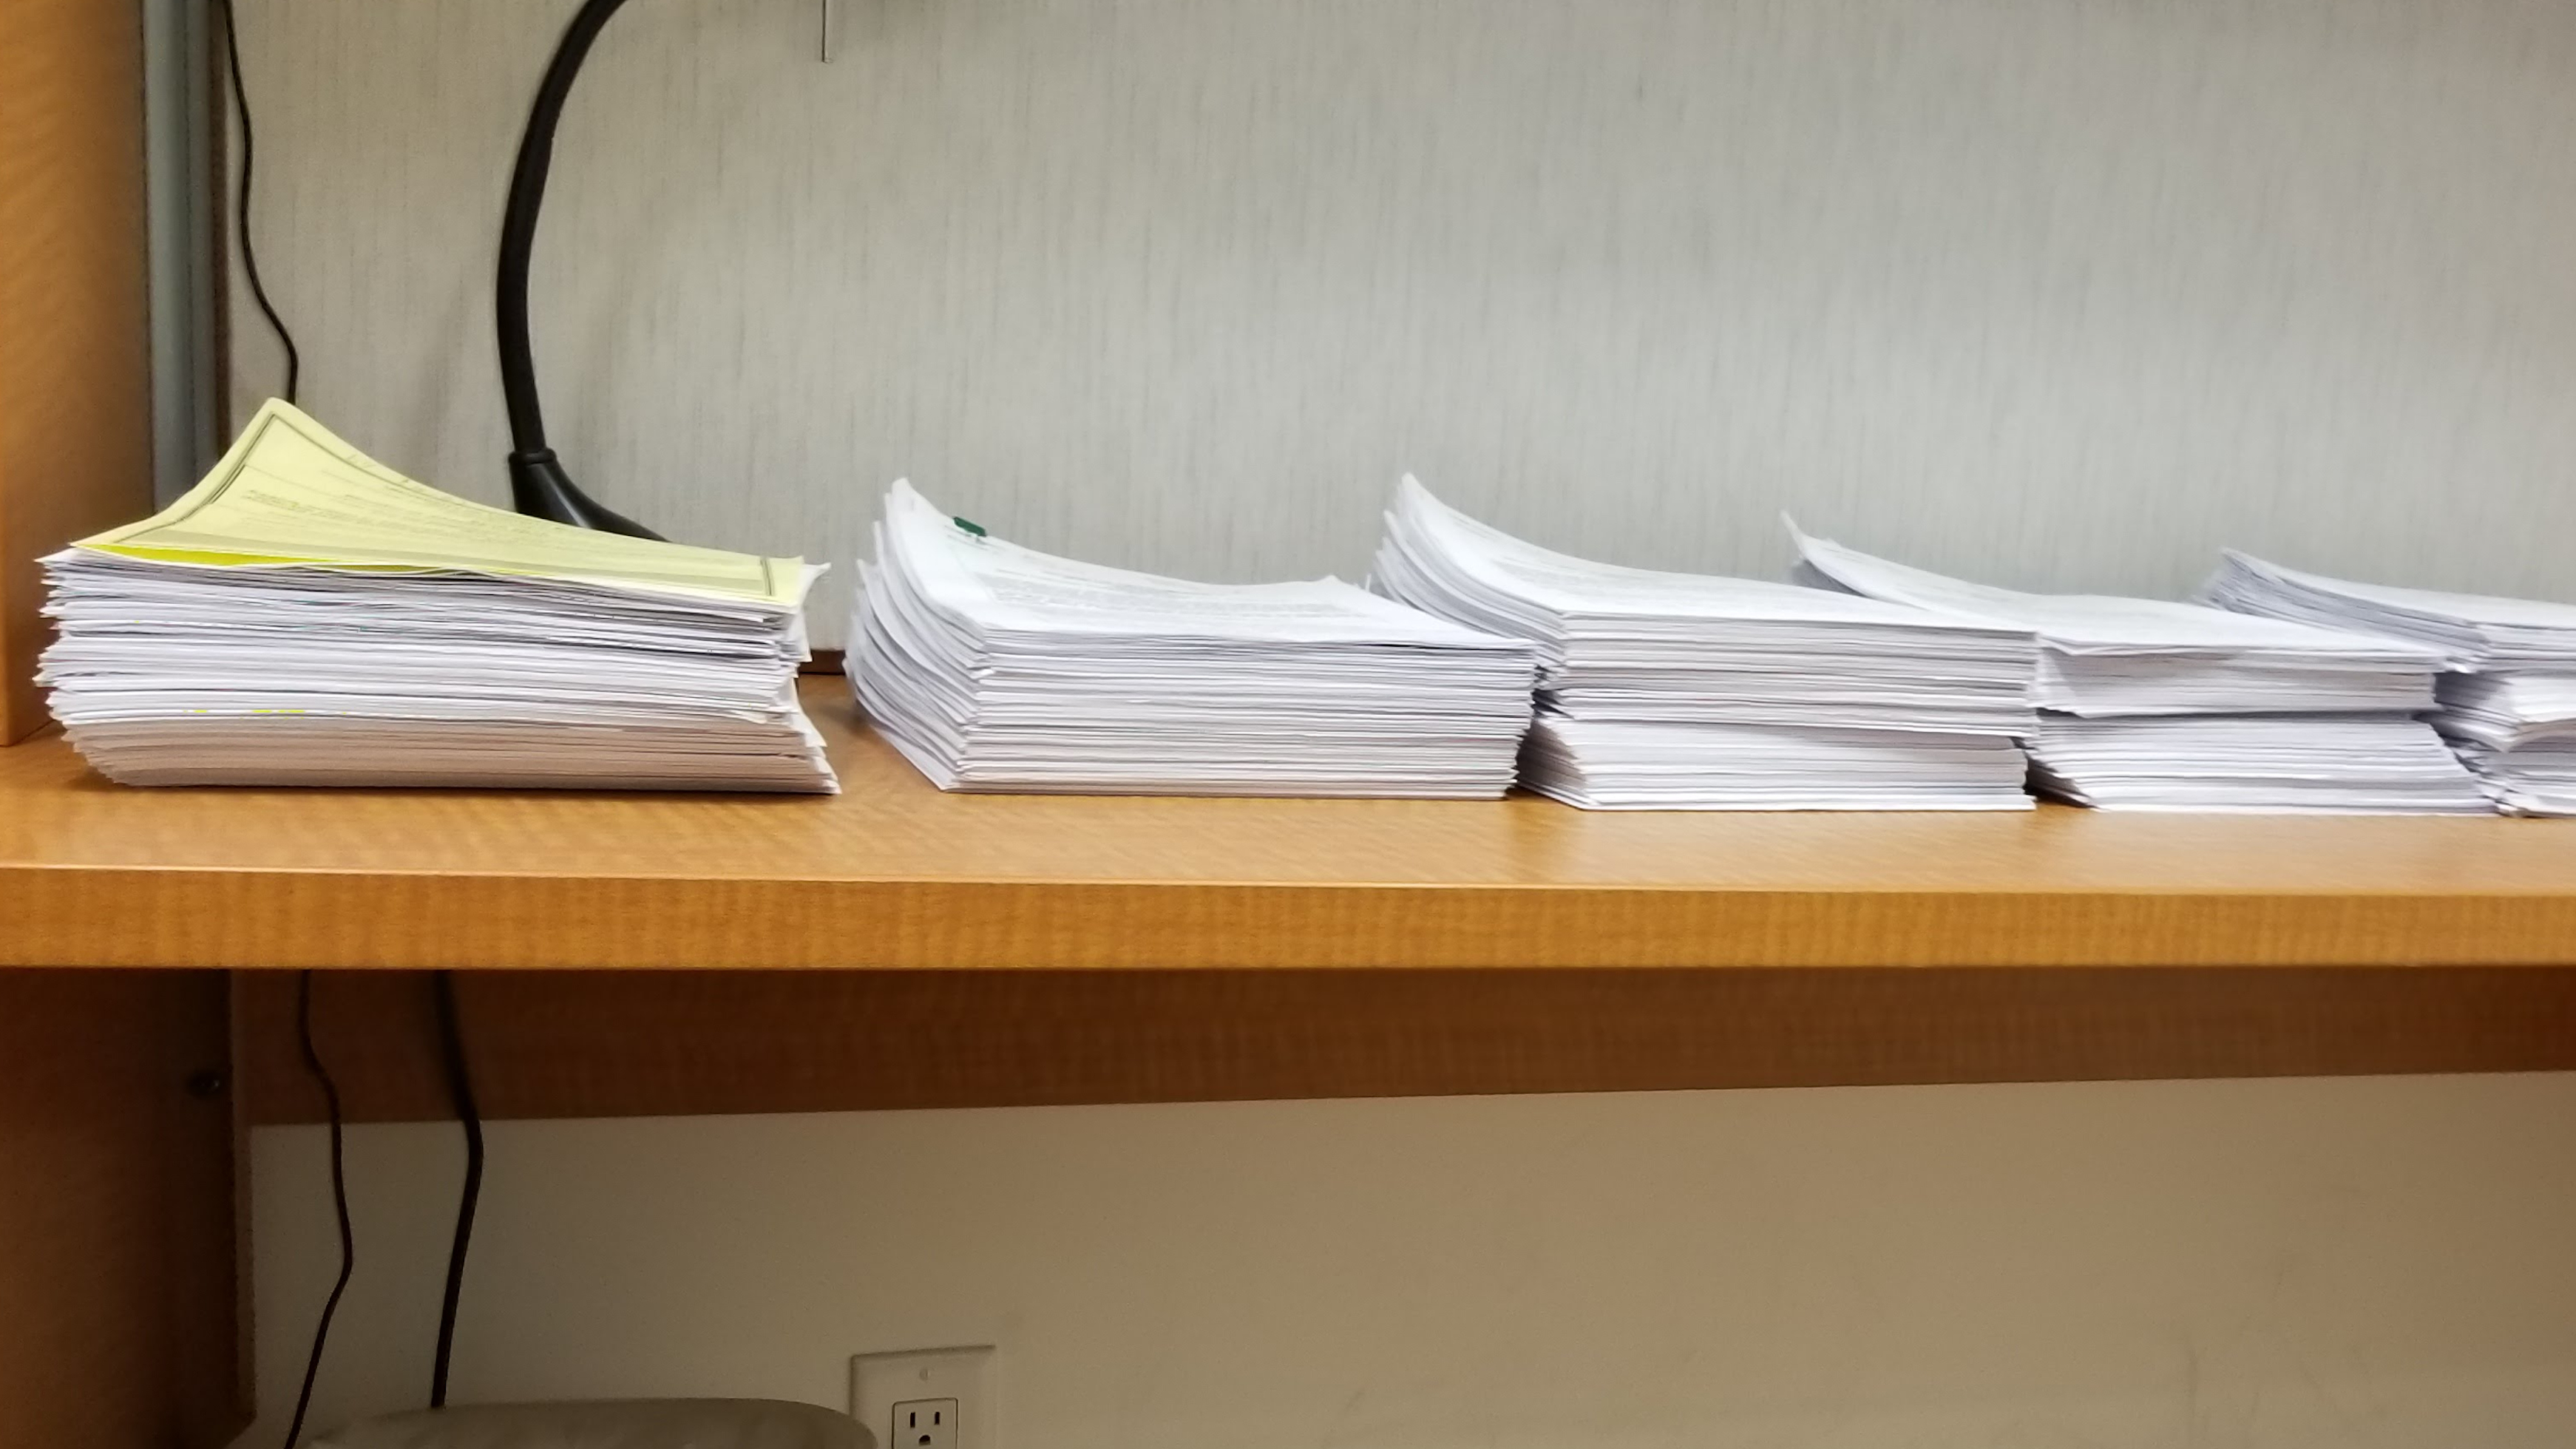
\includegraphics[width=\linewidth]{figs/test-papers.jpg}
\end{sbspanel}%
\end{sidebyside}%
\par
Can you think of an efficient way to count the papers?%
\par\smallskip%
\noindent\textbf{\blocktitlefont Hint}.\hypertarget{g:hint:id247544}{}\quad{}You wouldn't just count them one by one\textellipsis{}%
\end{inlineexercise}
In \hyperref[x:exercise:ex-counting-socks]{Checkpoint~{\xreffont\ref{x:exercise:ex-counting-socks}}} the problem of counting the total number of pairs of socks had a straightforward solution. Since the socks were already separated by colour, and you knew how many of each colour you had, you just had to add the number of pairs for each colour to get the total.%
\par
For the test papers in \hyperref[x:exercise:ex-counting-test-papers]{Checkpoint~{\xreffont\ref{x:exercise:ex-counting-test-papers}}} there are certainly multiple ways to do this. One method that TAs use is to form piles of ten, and count how many piles are produced. This is actually more similar to the socks example than you might think. Separating the huge pile of papers into groups of 10 has the same goal as separating socks by colour: one just has to add the numbers in each pile together in the end (which, if all piles have 10, is an easy calculation).%
\par
This is the \terminology{Sum Rule} in action.%
\begin{definition}{Partition.}{x:definition:def-partition}%
Let \(A\) be a finite set. We say that \(B_1,B_2,\ldots,B_m\) form a \terminology{partition} of \(A\) if%
\begin{itemize}[label=\textbullet]
\item{}\(B_i \cap B_j = \varnothing\) for all \(i \ne j\), and%
\item{}\(B_1 \cup B_2 \cup \cdots \cup B_m = A\).%
\end{itemize}
%
\end{definition}
\begin{principle}{Sum Rule.}{}{x:principle:prin-sum-rule}%
If \(B_1,B_2,\ldots,B_m\) form a partition of \(A\), then%
\begin{equation*}
|A| = \sum_{i=1}^n |B_i| = |B_1| + |B_2| + \cdots + |B_m|\text{.}
\end{equation*}
%
\end{principle}
The \hyperref[x:principle:prin-sum-rule]{Sum Rule} essentially tells us that in order to count a set of objects, we can break these objects up into disjoint cases, count each case separately, then add them all together in the end. Sounds reasonable!%
\begin{inlineexercise}{Twitter Followers.}{x:exercise:ex-counting-twitter}%
TJ is an avid Twitter user, where he manages the following accounts:%
\begin{itemize}[label=\textbullet]
\item{}A \href{https://twitter.com/tjyusun}{personal account} with 200 followers;%
\item{}A K-pop stan Twitter account with 2500 followers;%
\item{}A third account with 12000 followers that tweets a picture of a puppy every hour.%
\end{itemize}
Can you determine the total number of unique followers TJ has? Explain whether or not the \hyperref[x:principle:prin-sum-rule]{Sum Rule} is applicable to this problem.%
\par\smallskip%
\noindent\textbf{\blocktitlefont Hint}.\hypertarget{g:hint:id237402}{}\quad{}To apply the Sum Rule, one needs to have a partition.%
\end{inlineexercise}
When we need to count objects that are constructed by performing \emph{successive steps} or operations that are independent, we use the \alert{Product Rule}.%
\begin{principle}{Product Rule.}{}{x:principle:prin-prod-rule}%
If a certain operation takes \(k\) steps to accomplish, and if there are:%
\begin{itemize}[label=\textbullet]
\item{}\(r_1\) ways of performing step 1,%
\item{}\(r_2\) ways of performing step 2 (regardless of how step 1 was performed),%
\item{}\(r_3\) ways of performing step 3 (regardless of how step 2 was performed),%
\item{}and so on\textellipsis{}%
\end{itemize}
Then, there are%
\begin{equation*}
\prod_{i=1}^k r_i = r_1 \cdot r_2 \cdot \ldots \cdot r_k
\end{equation*}
ways of performing steps 1 to \(k\).%
\end{principle}
\begin{inlineexercise}{Counting Outfits.}{x:exercise:ex-counting-outfit}%
You are deciding what outfit to wear to your Zoom class today. You have been putting off doing laundry, so you only have 3 clean shirts and 3 clean pairs of pants. Also, you have 8 pairs of socks to choose from. How many different outfits can you wear to school today? (Assume you cannot go to school shirtless, but you can go pantless or barefoot\textemdash{}no one will see!)%
\end{inlineexercise}
\begin{inlineexercise}{Proof of the Product Rule.}{x:exercise:ex-counting-prove-product}%
Use the \hyperref[x:principle:prin-sum-rule]{Sum Rule} to prove the \hyperref[x:principle:prin-prod-rule]{Product Rule}.%
\par\smallskip%
\noindent\textbf{\blocktitlefont Hint}.\hypertarget{g:hint:id237797}{}\quad{}Induction on \(k\).%
\end{inlineexercise}
\begin{example}{Multiple Choice Exam.}{x:example:eg-counting-mcq}%
A multiple-choice exam has 20 questions and four choices for each question. How many possible combinations of responses are there?%
\begin{sidebyside}{1}{0.35}{0.35}{0}%
\begin{sbspanel}{0.3}%
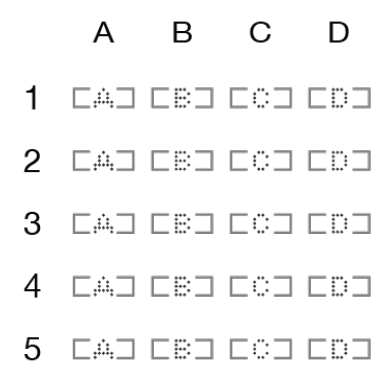
\includegraphics[width=\linewidth]{figs/mcq1.png}
\end{sbspanel}%
\end{sidebyside}%
\par\smallskip%
\noindent\textbf{\blocktitlefont Solution}.\hypertarget{g:solution:id237897}{}\quad{}Answering the whole test takes 20 individual, independent steps: picking one answer to each question. If we assume each question needs to have one answer, then in the statement of the \hyperref[x:principle:prin-prod-rule]{Product Rule}, \(r_1 = 4\), \(r_2 = 4\), and so on until \(r_{20} = 4\), giving a total of%
\begin{equation*}
\underbrace{4 \times 4 \times \cdots \times 4}_{\text{20 times}} = 4^{20}=1099511627776
\end{equation*}
possible answer combinations.%
\par
In other words, pure guessing as a strategy will on average result in a perfect score once every one trillion tries. In comparison, the odds of matching six numbers in Lotto 6\slash{}49 is much better: one in 14 million.%
\par
If we allow questions to be left unanswered, then there are \(5^{20}=95367431640625\), around 96 trillion possible ways to answer the test.%
\end{example}
\begin{inlineexercise}{Concert Seating with \(n\) people.}{x:exercise:ex-counting-coldplay2}%
Apply the Product Rule to answer (a) and (b) of \hyperref[x:exercise:ex-counting-coldplay]{Checkpoint~{\xreffont\ref{x:exercise:ex-counting-coldplay}}}, then generalize this method to count the number of ways to sit \(n\) people in a row of \(n\) seats.%
\end{inlineexercise}
Because the following operation frequently turns up in counting problems, we have a special name for it.%
\begin{definition}{Factorial.}{x:definition:def-factorial}%
For integer \(n \geq 0\), the \terminology{factorial} of \(n\), denoted by \(n!\), is%
\begin{equation*}
n! = \prod_{i=1}^n i = n \cdot (n-1) \cdot (n-2) \cdot \ldots \cdot 2 \cdot 1\text{.}
\end{equation*}
By convention we define \(0! = 1\).%
\label{x:notation:not-factorial}%
\end{definition}
\begin{remark}{}{x:remark:remark-factorial}%
For problems where the answer involves a factorial, it is fine to leave the factorial in your answer without computing the actual value.%
\end{remark}
\begin{example}{Dog Adoption, again.}{x:example:eg-counting-dogs-again}%
\hyperref[x:example:eg-counting-dogs]{Example~{\xreffont\ref{x:example:eg-counting-dogs}}} had too many combinations to list, but using the \hyperref[x:principle:prin-prod-rule]{Product Rule} we see that there are a total of%
\begin{equation*}
10! = 10 \times 9 \times 8 \times \cdots \times 1 = 3628800 \text{ combinations}\text{.}
\end{equation*}
%
\end{example}
%
%
\typeout{************************************************}
\typeout{Solutions 2.1.1 Solutions to Selected Checkpoints}
\typeout{************************************************}
%
\begin{solutions-subsection}{Solutions to Selected Checkpoints}{}{Solutions to Selected Checkpoints}{}{}{g:solutions:id238330}
\begin{inlineexercisesolution}{2.1.2}{Concert Seating.}{x:exercise:ex-counting-coldplay}
\textbf{\blocktitlefont Solution}.\hypertarget{g:solution:id247108-main}\quad{}a. Listing all possibilities yields 6 ways without any restrictions:%
\begin{sidebyside}{1}{0.1}{0.1}{0}%
\begin{sbspanel}{0.8}%
{\centering%
{\tabularfont%
\begin{tabular}{lll}
(Mina, Lisa, Wendy)&(Lisa, Wendy, Mina)&(Wendy, Mina, Lisa)\tabularnewline[0pt]
(Mina, Wendy, Lisa)&(Lisa, Mina, Wendy)&(Wendy, Lisa, Mina)
\end{tabular}
}%
\par}
\end{sbspanel}%
\end{sidebyside}%
\par
b. Exactly two of these seating arrangements has Lisa in the middle seat.%
\end{inlineexercisesolution}
\begin{inlineexercisesolution}{2.1.4}{Socks!}{x:exercise:ex-counting-socks}
\textbf{\blocktitlefont Solution}.\hypertarget{g:solution:id247454-main}\quad{}It's not a trick question. \(3 + 4 + 2 = 9\).%
\end{inlineexercisesolution}
\begin{inlineexercisesolution}{2.1.8}{Twitter Followers.}{x:exercise:ex-counting-twitter}
\textbf{\blocktitlefont Solution}.\hypertarget{g:solution:id237395-main}\quad{}If all followers among TJ's three accounts are different people, then we could just add%
\begin{equation*}
200 + 2500 + 12000 = 14700
\end{equation*}
to get the total number of unique followers. However this is very possibly not the case!%
\par
For instance, if we knew that a hundred of TJ's followers on his personal account also follow the puppy auto-tweeter, then the number of unique followers among all three accounts is no more than 14600. This is lower if there is more overlap.%
\par
The \hyperref[x:principle:prin-sum-rule]{Sum Rule}does not apply becase the three sets of followers do not form a \hyperref[x:definition:def-partition]{partition} of the set we want to count (the first condition fails).%
\end{inlineexercisesolution}
\begin{inlineexercisesolution}{2.1.10}{Counting Outfits.}{x:exercise:ex-counting-outfit}
\textbf{\blocktitlefont Solution}.\hypertarget{g:solution:id237625-main}\quad{}The operation of \emph{picking an outfit to wear to school} can be broken down into the following steps:%
\begin{enumerate}
\item{}Pick a shirt (3 choices)%
\item{}Pick a pair of pants (4 choices, including no pants; regardless of which shirt you picked)%
\item{}Pick a pair of socks (9 choices, including barefoot; regardless of which shirt\slash{}pants you wear)%
\end{enumerate}
So it takes 3 steps to decide on an outfit, where \(r_1 = 3\), \(r_2 = 4\), and \(r_3 = 9\). By the Product Rule, there are \(3 \cdot 4 \cdot 9 = 108\) different outfits you can choose to wear.%
\end{inlineexercisesolution}
\begin{inlineexercisesolution}{2.1.13}{Concert Seating with \(n\) people.}{x:exercise:ex-counting-coldplay2}
\textbf{\blocktitlefont Solution}.\hypertarget{g:solution:id238057-main}\quad{}We can generalize \hyperref[x:exercise:ex-counting-coldplay]{Checkpoint~{\xreffont\ref{x:exercise:ex-counting-coldplay}}}as follows: if \(n\) people want to sit in a row of \(n\) seats (with no restriction), then the whole operation of assigning seats to people takes \(n\) steps, where the first person has \(n\) seats to choose from, the next person has \(n-1\), and so on, until 1 seat is left for the last person. The Product Rule then gives a total number of%
\begin{equation*}
n \cdot (n-1) \cdot (n-2) \cdot \ldots \cdot 2 \cdot 1
\end{equation*}
ways that \(n\) people can sit in \(n\) seats in a row.%
\end{inlineexercisesolution}
\end{solutions-subsection}
\end{sectionptx}
%
%
\typeout{************************************************}
\typeout{Section 2.2 Permutations and Combinations}
\typeout{************************************************}
%
\begin{sectionptx}{Permutations and Combinations}{}{Permutations and Combinations}{}{}{x:section:sec-permutations-combinations}
\begin{objectives}{Objectives}{g:objectives:id238392}
%
\begin{itemize}[label=\textbullet]
\item{}Derive the formulas for permutations and combinations (of \(n\) objects taken \(k\) at a time), multi-permutations, and permutations with repetitions allowed.%
\item{}Given a word problem, recognize which of the above techniques is applicable, and use it to solve the problem.%
\end{itemize}
\end{objectives}
In this section we get a little bit fancier and define some special quantities that show up frequently when counting objects or rearrangements. First, recall that the \hyperref[x:definition:def-factorial]{factorial} of \(n\) is shorthand for the product%
\begin{equation*}
n! = n \times (n-1) \times \cdots \times 1\text{,}
\end{equation*}
which, as we saw in the previous section, can be used to count the number of ways to sit \(n\) people in a row for a concert.%
\begin{definition}{Permutation.}{x:definition:def-permutation}%
A \terminology{permutation} is a bijection from a finite set \(S\) to itself.%
\end{definition}
\begin{remark}{}{x:remark:remark-permutation}%
If \(|S| = n\), then there are \(n!\) bijections \(S \rightarrow S\). Equivalently,%
\begin{itemize}[label=\textbullet]
\item{}There are \(n!\) ways to arrange \(n\) \emph{distinct} objects in a row.%
\item{}There are \(n!\) rearrangements of a word with \(n\) \emph{distinct} letters. Each rearrangement is said to be a \emph{permutation} of the \(n\) letters.%
\end{itemize}
%
\end{remark}
\begin{example}{Counting Bijections.}{x:example:eg-counting-bijections}%
Let \(S = \{a,b,c,d\}\). Then the function \(f: S \rightarrow S\) defined by%
\begin{equation*}
f(a) = b, f(b) = d, f(c) = c, f(d) = a
\end{equation*}
is one example of a bijection from \(S\) to \(S\). Since \(|S| = 4\), there are a total of \(4! = 24\) bijections from \(S\) to itself.%
\end{example}
What if we wanted to rearrange \(k\) of the \(n\) distinct objects (i.e. only a subset)?%
\begin{inlineexercise}{EQUATION.}{x:exercise:ex-counting-EQUATION}%
How many four-letter words can be formed using the letters of the word%
\begin{sidebyside}{1}{0.4}{0.4}{0}%
\begin{sbspanel}{0.2}%
EQUATION?%
\end{sbspanel}%
\end{sidebyside}%
\par\smallskip%
\noindent\textbf{\blocktitlefont Hint}.\hypertarget{g:hint:id324929}{}\quad{}How many choices do you have for the first letter? the second? the others? Use the \hyperref[x:principle:prin-prod-rule]{Product Rule}.%
\end{inlineexercise}
Let's generalize this. Let \(k \leq n\), and use the \hyperref[x:principle:prin-prod-rule]{Product Rule} to count the number of ways to arrange \(k\) objects in a row, taking from a set of \(n\) distinct objects.%
\par
Then express your answer in terms of factorials, and complete the statement of \hyperref[x:proposition:prop-Pnk]{Proposition~{\xreffont\ref{x:proposition:prop-Pnk}}} below.%
\begin{proposition}{\(k\)-permutation of an \(n\)-set.}{}{x:proposition:prop-Pnk}%
If \(k \leq n\), then the number of permutations of \(k\) distinct elements from a set of size \(n\) is \fillin{9.090909090909092}.%
\end{proposition}
\begin{remark}{}{x:remark:remark-Pnk-notation}%
In some textbooks the above quantity is denoted by \(P(n,k)\) or \(_nP_k\). When solving problems you may use either notation and leave your answer in that form.%
\end{remark}
\begin{example}{Student Council Representatives.}{x:example:eg-counting-student-council}%
How many ways can a class of 45 students elect a president, vice-president, and secretary to represent them on student council?%
\par\smallskip%
\noindent\textbf{\blocktitlefont Solution}.\hypertarget{g:solution:id325312}{}\quad{}This corresponds to the number of permutations of 45 objects taken 3 at a time, so the total is%
\begin{equation*}
45 \cdot 44 \cdot 43 = 85140\text{.}
\end{equation*}
%
\par
One can also imagine the solution using the \hyperref[x:principle:prin-prod-rule]{Product Rule}: there are three steps to this operation:%
\begin{sidebyside}{1}{0.15}{0.15}{0}%
\begin{sbspanel}{0.7}%
{\centering%
{\tabularfont%
\begin{tabular}{ll}
elect a president:&45 choices\tabularnewline[0pt]
elect a vice-president:&44 choices\tabularnewline[0pt]
elect a secretary:&43 choices
\end{tabular}
}%
\par}
\end{sbspanel}%
\end{sidebyside}%
\par
Then the number of ways to do so is \(45 \cdot 44 \cdot 43\).%
\end{example}
\begin{inlineexercise}{ZAHLEN.}{x:exercise:ex-counting-ZAHLEN}%
%
\begin{enumerate}[label=(\alph*)]
\item{}Count the number of three-letter words that can be formed from the letters of the word ZAHLEN.%
\item{}How many of the words from (a) contain \alert{only consonants}?%
\item{}How many of the words from (a) contain \alert{contain exactly one vowel}?%
\end{enumerate}
%
\par\smallskip%
\noindent\textbf{\blocktitlefont Hint}.\hypertarget{g:hint:id325453}{}\quad{}For part c., try using the \hyperref[x:principle:prin-prod-rule]{Product Rule}. What steps need to be performed to form a word that satisfies the given condition?%
\par\smallskip%
\noindent\textbf{\blocktitlefont Answer}.\hypertarget{g:answer:id325513}{}\quad{}a. 120%
\par
b. 24%
\par
c. 72%
\end{inlineexercise}
The next example shows that having \emph{distinct} objects is crucial in the statement of \hyperref[x:definition:def-permutation]{Definition~{\xreffont\ref{x:definition:def-permutation}}}.%
\begin{example}{Repeated Letters.}{x:example:eg-counting-YEET}%
Count the number of arrangements of the letters in the word YEET.%
\par
\alert{Solution} A misguided attempt to apply \hyperref[x:definition:def-permutation]{Definition~{\xreffont\ref{x:definition:def-permutation}}} will yield \(4! = 24\) possible arrangements of the word YEET. However, we see that there are only 12 possibilities when we list them all:%
\begin{sidebyside}{1}{0.2}{0.2}{0}%
\begin{sbspanel}{0.6}%
{\centering%
{\tabularfont%
\begin{tabular}{llllll}
YEET&YETE&YTEE&TYEE&TEYE&TEEY\tabularnewline[0pt]
EETY&EEYT&ETYE&ETEY&EYET&EYTE
\end{tabular}
}%
\par}
\end{sbspanel}%
\end{sidebyside}%
\par
This is because the letters in the word YEET are \emph{not} distinct! If we distinguish each letter E in the word by calling them E\(_1\) and E\(_2\), then we see that each arrangement above actually came from \alert{two} arrangements, for instance:%
\begin{sidebyside}{1}{0.15}{0.15}{0}%
\begin{sbspanel}{0.7}%
{\centering%
{\tabularfont%
\begin{tabular}{l}
YE\(_1\)E\(_2\)T and YE\(_2\)E\(_1\)T \(\rightarrow\) YEET\tabularnewline[0pt]
YE\(_1\)TE\(_2\) and YE\(_2\)TE\(_1\) \(\rightarrow\) YETE
\end{tabular}
}%
\par}
\end{sbspanel}%
\end{sidebyside}%
\par
Thus while \hyperref[x:definition:def-permutation]{Definition~{\xreffont\ref{x:definition:def-permutation}}} predicts \(4! = 24\) arrangements of the four letters Y, E\(_1\), E\(_2\), and T, we see that for each arrangement either E\(_1\) is somewhere to the left, or somewhere to the right of E\(_2\). Hence we dividing by two to account for this overcounting, which gives the correct number, \(4!/2 = 12\).%
\end{example}
What if three letter E's are repeated? Following the same reasoning, we can distinguish them first as E\(_1\), E\(_2\), and E\(_3\), then apply \hyperref[x:definition:def-permutation]{Definition~{\xreffont\ref{x:definition:def-permutation}}}. We will get a number that overcounts the actual answer by a factor of 6 this time, since there are \(3! = 6\) ways to arrange the three E's:%
\begin{sidebyside}{6}{0.0233333333333333}{0.0233333333333333}{0.0466666666666667}%
\begin{sbspanel}{0.12}%
E\(_1\)E\(_2\)E\(_3\)%
\end{sbspanel}%
\begin{sbspanel}{0.12}%
\par
E\(_1\)E\(_3\)E\(_2\)%
\end{sbspanel}%
\begin{sbspanel}{0.12}%
\par
E\(_2\)E\(_1\)E\(_3\)%
\end{sbspanel}%
\begin{sbspanel}{0.12}%
\par
E\(_2\)E\(_3\)E\(_1\)%
\end{sbspanel}%
\begin{sbspanel}{0.12}%
\par
E\(_3\)E\(_1\)E\(_2\)%
\end{sbspanel}%
\begin{sbspanel}{0.12}%
\par
E\(_3\)E\(_2\)E\(_1\)%
\end{sbspanel}%
\end{sidebyside}%
\par
We generalize this to \hyperref[x:proposition:prop-perm-repeat]{Proposition~{\xreffont\ref{x:proposition:prop-perm-repeat}}}, which gives a way to count rearrangements of words when some letters are repeated. (We say the letters are elements of a \terminology{multiset}, which generalizes sets to allow for multiple instances of elements.)%
\begin{proposition}{Permutations of a multiset.}{}{x:proposition:prop-perm-repeat}%
Let \(S\) be a set with \(n\) (not necessarily distinct) objects, such that there are \(n_1\) objects of type 1, \(n_2\) objects of type 2, \(\ldots\), and \(n_k\) objects of type \(k\), where \(n_1 + n_2 + \cdots + n_k = n\). Then the number of arrangements of these objects is%
\begin{equation*}
\dfrac{n!}{n_1! n_2! \cdots n_k!}\text{.}
\end{equation*}
%
\end{proposition}
\begin{inlineexercise}{MISSISSAUGA.}{x:exercise:ex-counting-MISSISSAUGA}%
How many arrangements can be formed using the letters of the word%
\begin{sidebyside}{1}{0.375}{0.375}{0}%
\begin{sbspanel}{0.25}%
MISSISSAUGA?%
\end{sbspanel}%
\end{sidebyside}%
\par\smallskip%
\noindent\textbf{\blocktitlefont Answer}.\hypertarget{g:answer:id226880}{}\quad{}\(\dfrac{11!}{1!\ 2!\ 4!\ 2!\ 1!\ 1!} = \dfrac{11!}{2!\ 4!\ 2!} = 415800.\)%
\end{inlineexercise}
\begin{inlineexercise}{MATHEMATICS.}{x:exercise:ex-counting-MATHEMATICS}%
Count the number of ways the letters of the word MATHEMATICS can be arranged so that%
\begin{enumerate}[label=(\alph*)]
\item{}The two M's are beside each other.%
\item{}The two M's are \emph{not} beside each other.%
\item{}The word MATH appears somewhere in the arrangement.%
\end{enumerate}
%
\par\smallskip%
\noindent\textbf{\blocktitlefont Hint 1}.\hypertarget{g:hint:id226949}{}\quad{}a. Treat `MM' as a single object.%
\par\smallskip%
\noindent\textbf{\blocktitlefont Hint 2}.\hypertarget{g:hint:id226956}{}\quad{}b. How are parts a. and b. related?%
\par\smallskip%
\noindent\textbf{\blocktitlefont Hint 3}.\hypertarget{g:hint:id226966}{}\quad{}c. Treat `MATH' as a single object.%
\end{inlineexercise}
\begin{inlineexercise}{Esports Tournament.}{x:exercise:ex-counting-esports}%
UTM Athletics is sending a team of 7 players to represent the university at an Ontario e-sports tournament called \emph{The Provincial}. Suppose that a total of 30 students tried out for the team.%
\begin{enumerate}[label=(\alph*)]
\item{}How many possible teams can be formed from the students who tried out?%
\item{}Suppose further that there are different positions on the team, as follows%
\begin{itemize}[label=\textbullet]
\item{}1 carry player%
\item{}1 mid player%
\item{}1 offlane player%
\item{}2 support players%
\item{}2 reserve players%
\end{itemize}
How many possible teams can be formed from the students who tried out? Assume everyone who tried out can play every position. (Not usually the case in reality\textellipsis{})%
\end{enumerate}
%
\par\smallskip%
\noindent\textbf{\blocktitlefont Hint 1}.\hypertarget{g:hint:id227172}{}\quad{}a. Each student either makes the team, or doesn't. Express each possible team as a sequence of 30 labels, one for each student who tried out.%
\par\smallskip%
\noindent\textbf{\blocktitlefont Hint 2}.\hypertarget{g:hint:id227190}{}\quad{}b. Same with a., but with more labels to account for the different positions on the team.%
\end{inlineexercise}
The scenario in part (a) of \hyperref[x:exercise:ex-counting-esports]{Checkpoint~{\xreffont\ref{x:exercise:ex-counting-esports}}} is an example where the order in which the students are picked does not matter -{}-{} the team is just a collection (set) of 7 players. Here's a smaller example:%
\begin{example}{Picking Bridesmaids.}{x:example:eg-counting-bridesmaids}%
Adele is getting married soon, and due to space constraints at the venue, needs to pick exactly two of her five best friends (Mel B., Mel C., Emma, Geri, and Victoria) to be her bridesmaids. How many possible combinations are there?%
\par
\alert{Solution} Each combination of bridesmaids corresponds to a rearrangement of the symbols \(\circ \circ \times \times \times\), given a \emph{fixed} arrangement of the five names in a row; for instance, the arrangement%
\begin{sidebyside}{1}{0.225}{0.225}{0}%
\begin{sbspanel}{0.55}%
{\centering%
{\tabularfont%
\begin{tabular}{lllll}
Mel B.&Mel C.&Emma&Gerri&Victoria\tabularnewline[0pt]
\(\circ\)&\(\times\)&\(\times\)&\(\circ\)&\(\times\)
\end{tabular}
}%
\par}
\end{sbspanel}%
\end{sidebyside}%
\par
means that Mel B. and Gerri will be bridesmaids, while%
\begin{sidebyside}{1}{0.225}{0.225}{0}%
\begin{sbspanel}{0.55}%
{\centering%
{\tabularfont%
\begin{tabular}{lllll}
Mel B.&Mel C.&Emma&Gerri&Victoria\tabularnewline[0pt]
\(\times\)&\(\times\)&\(\times\)&\(\circ\)&\(\circ\)
\end{tabular}
}%
\par}
\end{sbspanel}%
\end{sidebyside}%
\par
corresponds to Geri and Victoria being chosen. Applying \hyperref[x:proposition:prop-perm-repeat]{Proposition~{\xreffont\ref{x:proposition:prop-perm-repeat}}} to the three \(\times\)'s and two \(\circ\)'s, we see that there are exactly \(\dfrac{5!}{2! 3!} = 10\) possible combinations.%
\par
\alert{Note} When the usual formula for \(k\)-permutations from an \(n\)-set (\hyperref[x:proposition:prop-Pnk]{Proposition~{\xreffont\ref{x:proposition:prop-Pnk}}})) is applied to the previous example, we get a total of \(\dfrac{5!}{(5-3)!} = 60\), which is incorrect. The reason is that this formula treats the pairs%
\begin{sidebyside}{3}{0.2}{0.2}{0}%
\begin{sbspanel}{0.25}%
(Geri, Victoria)%
\end{sbspanel}%
\begin{sbspanel}{0.1}%
\par
and%
\end{sbspanel}%
\begin{sbspanel}{0.25}%
\par
(Victoria, Geri)%
\end{sbspanel}%
\end{sidebyside}%
\par
as different outcomes, while for this example they both correspond to the same combination of \(\{\text{Geri}, \text{Victoria}\}\) being chosen as bridesmaids, since the order doesn't matter.%
\end{example}
\begin{assemblage}{Overcounting as a Counting Technique.}{x:assemblage:box-overcounting}%
In the previous examples you may have been reminded of the main difference between an \emph{\(n\)-tuple} \((a_1,a_2,\ldots,a_n)\) and a \emph{set of \(n\) elements} \(\{a_1,a_2,\ldots,a_n\}\): order.%
\par
To give a small example, the triples \((1,2,3)\) and \((3,1,2)\) are \emph{not} equal in \(\mathbb{R}^3\), and there are a total of six \emph{different} triples using these same numbers:%
\par
%
\begin{align*}
(1,2,3) \amp \amp (2,1,3) \amp \amp (3,1,2)\\
(1,3,2) \amp \amp (2,3,1) \amp \amp (3,2,1)
\end{align*}
%
\par
On the other hand, the sets \(\{1,2,3\}\) and \(\{3,2,1\}\) are equal\textemdash{}it doesn't matter how we write the three numbers since a set is defined by object membership.%
\par
In general, to count objects for which order does not matter, we can \alert{assume order matters first, then divide by the overcounting factor}, typically the factorial of how many elements are under consideration.%
\par
As another example, in \hyperref[x:proposition:prop-perm-repeat]{Proposition~{\xreffont\ref{x:proposition:prop-perm-repeat}}}, each \(n_i!\) term in the denominator is the overcounting factor associated with first treating all objects of type \(i\) (there are \(n_i\) of them) differently.%
\end{assemblage}
When selecting \(k\) elements from a set of \(n\), and if the order in which they are selected does not matter, we simply need to divide by \(k!\).%
\begin{definition}{Combination.}{x:definition:def-combination}%
A \terminology{combination} of \(k\) elements taken from a set \(S\) of size \(n\) is any \(k\)-element subset of \(S\).%
\end{definition}
\begin{proposition}{\(k\)-combinations of an \(n\)-set.}{}{x:proposition:prop-comb}%
The number of \(k\)-combinations of a set with \(n\) distinct elements, denoted by \(\displaystyle\binom{n}{k}\) (read as `\(n\) choose \(k\)'), is%
\begin{equation*}
\binom{n}{k} = \dfrac{n!}{(n-k)!\ k!} = \dfrac{{}_nP_k}{k!}\text{.}
\end{equation*}
Alternative notation for this include \(C(n,k)\) and \(_nC_k\).%
\end{proposition}
\begin{example}{Counting Cards.}{x:example:eg-counting-standard-deck}%
A \terminology{standard deck of cards} consists of 52 cards, which come in 13 ranks (A\slash{}ace, 2, 3, 4, 5, 6, 7, 8, 9, 10, J\slash{}jack, Q\slash{}queen, K\slash{}king) of four cards each, one for each suit: clubs \(\clubsuit\) (a black suit), spades \(\spadesuit\) (black), hearts \(\heartsuit\) (red), diamonds \(\diamondsuit\) (red).%
\begin{enumerate}[label=(\alph*)]
\item{}How many outcomes (or \alert{hands}) are possible when you draw five cards at random from the deck?%
\item{}How many of these five-card hands comprise only numbered cards?%
\item{}How many of these five-card hands have exactly two red and three black cards?%
\end{enumerate}
%
\par
\alert{Solution} a. There are 52 distinct cards in the deck, and we are drawing five of them at random. Each outcome only depends on which cards are drawn, so the order in which we draw them does not matter. Therefore there are%
\begin{equation*}
\binom{52}{5} = \frac{52!}{47! \ 5!} = 2598960
\end{equation*}
possible five-card hands.%
\par
b. The ranks 2 to 10 are the numbered cards; there are a total of 36 numbered cards in a deck (9 ranks times 4 suits each). The number of five-card hands drawn from these cards is%
\begin{equation*}
\binom{36}{5}\text{.}
\end{equation*}
%
\par
c. The process of forming such a five-card hand can be broken down into two steps:%
\begin{sidebyside}{2}{0.05}{0.05}{0.1}%
\begin{sbspanel}{0.4}%
Step 1: Pick two red cards%
\end{sbspanel}%
\begin{sbspanel}{0.4}%
\par
Step 2: Pick three black cards%
\end{sbspanel}%
\end{sidebyside}%
\par
These two steps are independent of one another. There are 26 black and 26 red cards, so the \hyperref[x:principle:prin-prod-rule]{Product Rule} tells us that there are%
\begin{equation*}
\binom{26}{2}\binom{26}{3}
\end{equation*}
five-card hands with this property.%
\end{example}
\begin{inlineexercise}{Esports Tournament, again.}{x:exercise:ex-counting-esports-comb}%
Solve part a. of \hyperref[x:exercise:ex-counting-esports]{Checkpoint~{\xreffont\ref{x:exercise:ex-counting-esports}}} using \hyperref[x:proposition:prop-comb]{Proposition~{\xreffont\ref{x:proposition:prop-comb}}}%
\par
Then solve part b. (and express your answer) using only combinations.%
\par\smallskip%
\noindent\textbf{\blocktitlefont Answer}.\hypertarget{g:answer:id332422}{}\quad{}b. Use the \hyperref[x:principle:prin-prod-rule]{Product Rule} where each step corresponds to selecting players for a role.%
\end{inlineexercise}
\begin{exploration}{Early Combinatorics.}{x:exploration:expl-susruta}%
Some of the earliest mentions of permutations and combinations occur in ancient Hindu texts dating back to the year 600 BC. Called \emph{vikalpa} and \emph{bhaṅga}, respectively, they were used in the study of \href{https://en.wikipedia.org/wiki/Sanskrit_prosody}{Vedic meters} in poetry, in architecture, in medicine, astrology, and other areas.%
\par
The following examples are taken from \hyperlink{x:biblio:bib-kolachana-2019}{[{\xreffont 2}]}.%
\begin{enumerate}[font=\bfseries,label=(\alph*),ref=\alph*]
\item{}The \href{https://en.wikipedia.org/wiki/Sushruta_Samhita}{\pubtitle{Suśruta-saṃhitā}}, (est. 500 BC) an ancient Hindu text on medicine and surgery, counts the number of combinations of the flavours \emph{sweet}, \emph{acid}, \emph{saline}, \emph{pungent}, \emph{bitter}, and \emph{astringent} taken two at a time, in the following way:%
\begin{quote}%
``On making two combinations in successive way, those beginning with sweet are found to be 5 in number; those beginning with acid are 4; those with saline 3; those with pungent 2; bitter and astringent make 1 combination.''%
\nopagebreak\par%
\hfill\textemdash{}{\setlength{\tabcolsep}{0pt}\begin{tabular}[t]{l@{}}
\pubtitle{Suśruta-saṃhitā} lxiii, as cited in \hyperlink{x:biblio:bib-kolachana-2019}{[{\xreffont 2}]}, p. 358
\end{tabular}}\\\par
\end{quote}
Explain how this computation shows that \(\displaystyle\binom{6}{2} = 15\).%
\item{}This excerpt from the \pubtitle{Anuyogadvāra-sūtra} (c. 500) explains how to compute \(6!\).%
\begin{quote}%
``What is the direct arrangement? Dharmāstikāya, Adharmāstikāya, Ākāśāstikāya, Jīvāstikāya, Pudgalāstikāya and Addhāsamaya—this is the direct arrangement. What is the reverse arrangement? Ad- dhāsamaya, Pudgalāstikāya, Jīvāstikāya, Ākāśāstikāya, Adharmā- stikāya, and Dharmāstikāya—this is the reverse arrangement. What are the mixed arrangements? From the series of numbers begin- ning with one and increasing by one up to six terms. The mutual products of these minus 2 will give the number of mixed arrange- ments.''%
\nopagebreak\par%
\hfill\textemdash{}{\setlength{\tabcolsep}{0pt}\begin{tabular}[t]{l@{}}
\pubtitle{Anuyogadvāra-sūtra}, Sūtra 97, as cited in \hyperlink{x:biblio:bib-kolachana-2019}{[{\xreffont 2}]}, p. 363.
\end{tabular}}\\\par
\end{quote}
Discuss what \emph{mixed arrangement} refers to and how the computation is carried out.%
\end{enumerate}
\end{exploration}
%
%
\typeout{************************************************}
\typeout{Solutions 2.2.1 Solutions to Selected Checkpoints}
\typeout{************************************************}
%
\begin{solutions-subsection}{Solutions to Selected Checkpoints}{}{Solutions to Selected Checkpoints}{}{}{g:solutions:id318337}
\begin{inlineexercisesolution}{2.2.8}{ZAHLEN.}{x:exercise:ex-counting-ZAHLEN}
\textbf{\blocktitlefont Solution}.\hypertarget{g:solution:id325573-main}\quad{}c. First, pick two consonants out of the four: \(_4P_2\) two-letter words can be formed. Then, pick a vowel (2 choices), and insert it into the two-letter word (3 possible slots) to form the required three-letter word with exactly one vowel. Thus the total number of such words is%
\begin{equation*}
_4P_2 \times 2 \times 3 = 72\text{.}
\end{equation*}
%
\end{inlineexercisesolution}
\begin{inlineexercisesolution}{2.2.12}{MATHEMATICS.}{x:exercise:ex-counting-MATHEMATICS}
\textbf{\blocktitlefont Solution}.\hypertarget{g:solution:id226988-main}\quad{}c. Treating `MATH' as a single object, we reduce the problem to counting the number of arrangements of eight distinct objects:%
\begin{sidebyside}{8}{0.02375}{0.02375}{0.0475}%
\begin{sbspanel}{0.13}%
`MATH'%
\end{sbspanel}%
\begin{sbspanel}{0.07}%
\par
E%
\end{sbspanel}%
\begin{sbspanel}{0.07}%
\par
M%
\end{sbspanel}%
\begin{sbspanel}{0.07}%
\par
A%
\end{sbspanel}%
\begin{sbspanel}{0.07}%
\par
T%
\end{sbspanel}%
\begin{sbspanel}{0.07}%
\par
I%
\end{sbspanel}%
\begin{sbspanel}{0.07}%
\par
C%
\end{sbspanel}%
\begin{sbspanel}{0.07}%
\par
S%
\end{sbspanel}%
\end{sidebyside}%
\par
Hence there are \(8!\) rearrangements of MATHEMATICS where the word MATH appears.%
\end{inlineexercisesolution}
\begin{inlineexercisesolution}{2.2.18}{Esports Tournament, again.}{x:exercise:ex-counting-esports-comb}
\textbf{\blocktitlefont Solution}.\hypertarget{g:solution:id332472-main}\quad{}First, we select the carry player: there are \(\displaystyle\binom{30}{1}\) ways to do so.%
\par
Then we can select the mid player in \(\displaystyle\binom{29}{1}\) ways regardless of who was picked to be carry. (Pick one player out of the 29 remaining.)%
\par
The offlane player can be picked in \(\displaystyle\binom{28}{1}\) ways.%
\par
To pick supports, \(\displaystyle\binom{27}{2}\) possible combinations. Selecting reserve players, \(\displaystyle\binom{25}{2}\) choices.%
\par
Hence there are%
\begin{equation*}
\binom{30}{1}\binom{29}{1}\binom{28}{1}\binom{27}{2}\binom{25}{2}
\end{equation*}
possible team combinations.%
\end{inlineexercisesolution}
\end{solutions-subsection}
\end{sectionptx}
%
%
\typeout{************************************************}
\typeout{Section 2.3 Binomial Coefficients}
\typeout{************************************************}
%
\begin{sectionptx}{Binomial Coefficients}{}{Binomial Coefficients}{}{}{x:section:sec-binomial-coefficients}
This is a longer sentence that is followed by another sentence. Two sentences, and a second paragraph to follow.%
\end{sectionptx}
%
%
\typeout{************************************************}
\typeout{Section 2.4 The Balls in Bins Formula}
\typeout{************************************************}
%
\begin{sectionptx}{The Balls in Bins Formula}{}{The Balls in Bins Formula}{}{}{x:section:sec-balls-in-bins}
This is a longer sentence that is followed by another sentence. Two sentences, and a second paragraph to follow.%
\end{sectionptx}
%
%
\typeout{************************************************}
\typeout{Section 2.5 Combinatorial Arguments}
\typeout{************************************************}
%
\begin{sectionptx}{Combinatorial Arguments}{}{Combinatorial Arguments}{}{}{x:section:sec-combinatorial-arguments}
This is a longer sentence that is followed by another sentence. Two sentences, and a second paragraph to follow.%
\end{sectionptx}
%
%
\typeout{************************************************}
\typeout{Exercises 2.6 Exercises}
\typeout{************************************************}
%
\begin{exercises-section}{Exercises}{}{Exercises}{}{}{x:exercises:exercises-counting}
\begin{introduction}{}%
Hello%
\end{introduction}%
\begin{divisionexercise}{1}{}{}{g:exercise:id318694}%
A \terminology{straight} is a hand of five different ranks in consecutive order. For example:%
\begin{sidebyside}{1}{0.3}{0.3}{0}%
\begin{sbspanel}{0.4}%
4\(\diamondsuit\) 5\(\heartsuit\) 6\(\clubsuit\) 7\(\clubsuit\) 8\(\diamondsuit\).%
\end{sbspanel}%
\end{sidebyside}%
\par
Assume that straights can start with an ace (A-2-3-4-5) or 10 (10-J-Q-K-A) or any other numbered card, but not with any face card (J, Q, or K). How many straights can be formed?%
\end{divisionexercise}%
\begin{divisionexercise}{2}{}{}{g:exercise:id319236}%
A \terminology{flush} is a hand of five cards, all of the same suit. For example, the five-card hand%
\begin{sidebyside}{1}{0.3}{0.3}{0}%
\begin{sbspanel}{0.4}%
4\(\spadesuit\) 5\(\spadesuit\) 8\(\spadesuit\) J\(\spadesuit\) K\(\spadesuit\)%
\end{sbspanel}%
\end{sidebyside}%
\par
is a flush.%
\par
%
\begin{enumerate}[label=(\alph*)]
\item{}How many flushes can be formed?%
\item{}How many flushes are also straights? (This hand is called a \terminology{straight flush}.)%
\end{enumerate}
%
\par\smallskip%
\noindent\textbf{\blocktitlefont Hint}.\hypertarget{g:hint:id319559}{}\quad{}LOL%
\end{divisionexercise}%
\end{exercises-section}
\end{chapterptx}
%
%
\typeout{************************************************}
\typeout{Chapter 3 Pigeonhole and Inclusion-Exclusion}
\typeout{************************************************}
%
\begin{chapterptx}{Pigeonhole and Inclusion-Exclusion}{}{Pigeonhole and Inclusion-Exclusion}{}{}{x:chapter:chap-principles}
\begin{introduction}{}%
Short intro here%
\end{introduction}%
%
%
\typeout{************************************************}
\typeout{Section 3.1 The Pigeonhole Principle}
\typeout{************************************************}
%
\begin{sectionptx}{The Pigeonhole Principle}{}{The Pigeonhole Principle}{}{}{x:section:sec-pigeonhole}
This is a longer sentence that is followed by another sentence. Two sentences, and a second paragraph to follow.%
\end{sectionptx}
%
%
\typeout{************************************************}
\typeout{Section 3.2 Principle of Inclusion-Exclusion}
\typeout{************************************************}
%
\begin{sectionptx}{Principle of Inclusion-Exclusion}{}{Principle of Inclusion-Exclusion}{}{}{x:section:sec-inclusion-exclusion}
This is a longer sentence that is followed by another sentence. Two sentences, and a second paragraph to follow.%
\end{sectionptx}
%
%
\typeout{************************************************}
\typeout{Exercises 3.3 Exercises}
\typeout{************************************************}
%
\begin{exercises-section}{Exercises}{}{Exercises}{}{}{x:exercises:exercises-principles}
\begin{introduction}{}%
Hello%
\end{introduction}%
\begin{divisionexercise}{1}{}{}{g:exercise:id319925}%
Pigeonhole stuff%
\end{divisionexercise}%
\begin{divisionexercise}{2}{}{}{g:exercise:id319940}%
Second question%
\par\smallskip%
\noindent\textbf{\blocktitlefont Hint}.\hypertarget{g:hint:id319944}{}\quad{}LOL%
\end{divisionexercise}%
\end{exercises-section}
\end{chapterptx}
%
%% A lineskip in table of contents as transition to appendices, backmatter
\addtocontents{toc}{\vspace{\normalbaselineskip}}
%
%
%
\typeout{************************************************}
\typeout{Appendix A Notation}
\typeout{************************************************}
%
%
\appendix
%
\begin{appendixptx}{Notation}{}{Notation}{}{}{x:appendix:app-notation}
\begin{longtable}[l]{lp{0.60\textwidth}r}
\addtocounter{table}{-1}
\textbf{Symbol}&\textbf{Description}&\textbf{Page}\\[1em]
\endfirsthead
\textbf{Symbol}&\textbf{Description}&\textbf{Page}\\[1em]
\endhead
\multicolumn{3}{r}{(Continued on next page)}\\
\endfoot
\endlastfoot
\(A \subseteq B\)&set inclusion&\pageref{g:notation:id235689}\\
\(\mathbb{N}\)&natural numbers&\pageref{g:notation:id322580}\\
\(\mathbb{Z}\)&integers&\pageref{g:notation:id322569}\\
\(\mathbb{Q}\)&rational numbers&\pageref{g:notation:id322592}\\
\(\mathbb{R}\)&real numbers&\pageref{g:notation:id322616}\\
\((a,b), [a,b], \text{etc.}\)&intervals of real numbers&\pageref{g:notation:id322611}\\
\(f: A \rightarrow B\)&function&\pageref{g:notation:id322729}\\
\((g \circ f)(x)\)&function composition&\pageref{g:notation:id322963}\\
\(|A| = |B|\)&cardinality, equal&\pageref{g:notation:id323012}\\
\(|A| \leq |B|\)&cardinality, less than&\pageref{g:notation:id323008}\\
\(P(A)\)&power set&\pageref{g:notation:id323197}\\
\(b \mid a\)&divides; divisible by&\pageref{g:notation:id322041}\\
\(\gcd(a,b)\)&greatest common divisor&\pageref{g:notation:id322505}\\
\(n!\)&factorial&\pageref{x:notation:not-factorial}\\
\end{longtable}
\end{appendixptx}
%
%
\typeout{************************************************}
\typeout{Appendix B List of Results}
\typeout{************************************************}
%
\begin{appendixptx}{List of Results}{}{List of Results}{}{}{x:appendix:app-definitions-theorems}
\noindent
\begin{longtable}[l]{ll}
\addtocounter{table}{-1}
\endfirsthead
\endhead
\multicolumn{2}{r}{(Continued on next page)}\\
\endfoot
\endlastfoot
\multicolumn{2}{l}{\null}\\[1.5ex] \multicolumn{2}{l}{\large Section 1.1 Sets and Functions}\\[0.5ex]
\hyperref[x:definition:def-set-inclusion-equality]{Definition 1.1.1}& Set Inclusion and Equality\\
\hyperref[x:definition:def-function]{Definition 1.1.4}& Function\\
\hyperref[x:definition:def-injective]{Definition 1.1.5}& Injective, surjective, bijective\\
\hyperref[x:definition:def-composition]{Definition 1.1.7}& Composition\\
\hyperref[x:theorem:thm-composition-of-bijections]{Theorem 1.1.8}& Properties of Compositions\\
\hyperref[x:definition:def-cardinality]{Definition 1.1.10}& Cardinality Relations\\
\hyperref[x:definition:def-power-set]{Definition 1.1.12}& Power Set\\
\multicolumn{2}{l}{\null}\\[1.5ex] \multicolumn{2}{l}{\large Section 1.2 Logic and Proof Techniques}\\[0.5ex]
\hyperref[x:theorem:thm-induction]{Theorem 1.2.1}& Principle of Mathematical Induction\\
\multicolumn{2}{l}{\null}\\[1.5ex] \multicolumn{2}{l}{\large Section 1.3 Integers and Divisibility}\\[0.5ex]
\hyperref[x:definition:def-divisibility]{Definition 1.3.1}& Divisibility and Primes\\
\hyperref[x:theorem:thm-division-algorithm]{Theorem 1.3.2}& Division Algorithm\\
\hyperref[x:definition:def-gcd]{Definition 1.3.4}& GCD\\
\hyperref[x:theorem:thm-bezout]{Theorem 1.3.6}& Bezout's Identity\\
\hyperref[x:lemma:lem-euclid]{Lemma 1.3.10}& Euclid's Lemma\\
\multicolumn{2}{l}{\null}\\[1.5ex] \multicolumn{2}{l}{\large Section 2.1 The Basic Counting Principles}\\[0.5ex]
\hyperref[x:definition:def-partition]{Definition 2.1.6}& Partition\\
\hyperref[x:definition:def-factorial]{Definition 2.1.14}& Factorial\\
\multicolumn{2}{l}{\null}\\[1.5ex] \multicolumn{2}{l}{\large Section 2.2 Permutations and Combinations}\\[0.5ex]
\hyperref[x:definition:def-permutation]{Definition 2.2.1}& Permutation\\
\hyperref[x:proposition:prop-Pnk]{Proposition 2.2.5}& \(k\)-permutation of an \(n\)-set\\
\hyperref[x:proposition:prop-perm-repeat]{Proposition 2.2.10}& Permutations of a multiset\\
\hyperref[x:definition:def-combination]{Definition 2.2.15}& Combination\\
\hyperref[x:proposition:prop-comb]{Proposition 2.2.16}& \(k\)-combinations of an \(n\)-set\\
\end{longtable}
\end{appendixptx}
%
%
\typeout{************************************************}
\typeout{Appendix C Solutions to Selected Exercises}
\typeout{************************************************}
%
\begin{solutions-chapter}{Solutions to Selected Exercises}{}{Solutions to Selected Exercises}{}{}{g:solutions:id320129}
\par\smallskip
\noindent\textbf{\Large{}2\space\textperiodcentered\space{}Counting Techniques}
\par\smallskip
\par\smallskip
\noindent\textbf{\Large{}2.6\space\textperiodcentered\space{}Exercises}
\par\smallskip
\begin{divisionsolution}{2.6.1}{}{g:exercise:id318694}%
\textbf{\blocktitlefont Solution}.\hypertarget{g:solution:id319184-back}\quad{}Test%
\end{divisionsolution}%
\begin{divisionsolution}{2.6.2}{}{g:exercise:id319236}%
\textbf{\blocktitlefont Solution}.\hypertarget{g:solution:id319602-back}\quad{}Hmmmm...%
\end{divisionsolution}%
\par\smallskip
\noindent\textbf{\Large{}3\space\textperiodcentered\space{}Pigeonhole and Inclusion-Exclusion}
\par\smallskip
\par\smallskip
\noindent\textbf{\Large{}3.3\space\textperiodcentered\space{}Exercises}
\par\smallskip
\begin{divisionsolution}{3.3.1}{}{g:exercise:id319925}%
\textbf{\blocktitlefont Solution}.\hypertarget{g:solution:id319938-back}\quad{}Lol%
\end{divisionsolution}%
\begin{divisionsolution}{3.3.2}{}{g:exercise:id319940}%
\textbf{\blocktitlefont Solution}.\hypertarget{g:solution:id319960-back}\quad{}Joke%
\end{divisionsolution}%
\end{solutions-chapter}
%
\backmatter
%
%
%
\typeout{************************************************}
\typeout{References  References}
\typeout{************************************************}
%
\begin{references-chapter-numberless}{References}{}{References}{}{}{g:references:id320106}
Fuchs, S., 2017. MAT102H5 Introduction to Mathematical Proofs. (Course Notes)Kolachana, A., Mahesh, K., Ramasubramanian, K., 2019. \href{https://doi.org/10.1007/978-981-13-7326-8_18}{Use of permutations and combinations in India}, in: Kolachana, A., Mahesh, K., Ramasubramanian, K. (Eds.), Studies in Indian Mathematics and Astronomy: Selected Articles of Kripa Shankar Shukla. Springer Singapore, Singapore, pp. 356–376.Wilson, R., Watkins, J.J., 2013. Combinatorics: Ancient \& Modern. OUP Oxford.\end{references-chapter-numberless}
\end{document}